\documentclass[12pt,a4paper]{report}

% ============================================================
% PACKAGES & PREAMBLE
% ============================================================
\usepackage[top=20mm, left=20mm, bottom=30mm, right=20mm, footskip=12mm]{geometry}
\usepackage{times}
\usepackage{setspace}
\usepackage{titlesec}
\usepackage{fancyhdr}
\usepackage{booktabs}
\usepackage{array}
\usepackage{longtable}
\usepackage{graphicx}
\usepackage{listings}
\usepackage{url}
\usepackage{hyperref}
\usepackage{indentfirst}
\usepackage{caption}
\usepackage{tocloft}
\usepackage{enumitem}
\usepackage{multirow}
\usepackage{eso-pic}
\urlstyle{rm}
\usepackage{tikz}
\usetikzlibrary{positioning, arrows.meta, shapes.geometric, calc}
\usepackage{pgfgantt}
\usepackage{amsmath} % For \numberwithin

\numberwithin{figure}{subsection}
\numberwithin{table}{subsection}

\onehalfspacing
\setlength{\parindent}{2.5em}

% Define mainmatter style (Chapter 1 onwards)
\fancypagestyle{mainmatter}{
  \fancyhf{}
  \fancyhead[C]{\fontsize{10}{12}\selectfont \textbf{RivetDB: A High-Performance Key-Value Store}}
  \fancyfoot[R]{\fontsize{10}{12}\selectfont \thepage}
  \fancyfoot[L]{\fontsize{10}{12}\selectfont SITS Narhe Pune-41(E\&TC Engineering)}
  \renewcommand{\headrule}{%
    \vspace{4pt}%
    \hrule height 2pt width \headwidth
    \vspace{1.5pt}%
    \hrule height 0.5pt width \headwidth
    \vspace{-8pt}%
  }
  \renewcommand{\footrule}{%
    \vspace{-4pt}%
    \hrule height 0.5pt width \headwidth
    \vspace{1.5pt}%
    \hrule height 2pt width \headwidth
    \vspace{4pt}%
  }
}

% Define frontmatter style (for abstract, TOC, etc. - EMPTY)
\fancypagestyle{frontmatter}{
  \fancyhf{}
  \renewcommand{\headrulewidth}{0pt}
  \renewcommand{\footrulewidth}{0pt}
}

% Force LaTeX's default 'plain' style to match frontmatter (for TOC, LOF, LOT - EMPTY)
\fancypagestyle{plain}{
  \fancyhf{}
  \renewcommand{\headrulewidth}{0pt}
  \renewcommand{\footrulewidth}{0pt}
}

% Section format
\titleformat{\section}
  {\normalfont\fontsize{12}{14}\bfseries}
  {\thesection}{1em}{\MakeUppercase}
\titlespacing*{\section}{0pt}{24pt}{12pt}

\titleformat{\subsection}
  {\normalfont\fontsize{12}{14}\bfseries}
  {\thesubsection}{1em}{}
\titlespacing*{\subsection}{0pt}{12pt}{6pt}

\lstset{
  basicstyle=\ttfamily\small,
  breaklines=true,
  frame=single,
  language=SQL,
  keywordstyle=\bfseries,
}
\captionsetup{font={normalsize}, labelfont={bf}}
\hypersetup{colorlinks=true, linkcolor=black, citecolor=black, urlcolor=blue}

% TOC formatting
\renewcommand{\cftchapfont}{\normalfont}
\renewcommand{\cftchappagefont}{\normalfont}
\renewcommand{\bibname}{}

\newcommand{\customchapter}[1]{
  \clearpage
  \pagestyle{mainmatter}
  \thispagestyle{empty}
  \refstepcounter{chapter}
  \addcontentsline{toc}{chapter}{\protect\numberline{\thechapter}#1}
  \vspace*{\fill}
  \begin{center}
    {\fontsize{14}{16}\selectfont\textbf{CHAPTER \thechapter}} \\[0.5\baselineskip]
    {\fontsize{12}{14}\selectfont\textbf{\MakeUppercase{#1}}}
  \end{center}
  \vspace*{\fill}
  \clearpage
  \vspace*{-14pt}
  {\centering \fontsize{12}{14}\selectfont\textbf{\MakeUppercase{#1}}\par}
  \addvspace{14pt}
}

\begin{document}

\pagenumbering{Roman} % I, II, III...
\pagestyle{frontmatter} % Apply front matter style

% ============================================================
% TITLE PAGE (I)
% ============================================================
\begin{titlepage}
\thispagestyle{empty} % No header/footer on title page
\begin{center}
\vspace*{1cm}
{\fontsize{12}{14}\selectfont \textbf{A}} \\
{\fontsize{12}{14}\selectfont \textbf{PROJECT REPORT ON}} \\
{\fontsize{14}{16}\selectfont \textcolor{cyan}{\textbf{``RIVETDB: A CONCURRENT, FEATURE-RICH IN-MEMORY DATABASE IN RUST WITH BUILT-IN TIME-SERIES, SQL QUERY, AND MULTI-TENANCY SUPPORT''}}} \\
\vspace{0.8cm}

{\fontsize{10}{12}\selectfont \textbf{SUBMITTED TO THE SAVITRIBAI PHULE PUNE}} \\
{\fontsize{10}{12}\selectfont \textbf{UNIVERSITY, PUNE IN THE PARTIAL FULFILLMENT FOR}} \\
{\fontsize{10}{12}\selectfont \textbf{THE AWARD OF THE DEGREE}} \\
{\fontsize{10}{12}\selectfont \textbf{OF}} \\
\vspace{0.8cm}

{\fontsize{14}{16}\selectfont \textbf{BACHELOR OF ENGINEERING}} \\
{\fontsize{14}{16}\selectfont \textbf{(ELECTRONICS AND TELECOMMUNICATION)}} \\
\vspace{0.8cm}

{\fontsize{12}{14}\selectfont \textbf{BY}} \\
\vspace{0.5cm}

\begin{tabular}{c@{\hspace{2cm}}c}
{\fontsize{12}{14}\selectfont \textbf{Name of Student}} & {\fontsize{12}{14}\selectfont \textbf{Exam Seat No.}} \\[0.5\baselineskip]
\textbf{Mr. Jatin Shimpi} & \textbf{B400570214} \\
\textbf{Mr. Ayan Shaikh} & \textbf{B400570185} \\
\textbf{Mr. Rahul Polas} & \textbf{B400570189} \\
\textbf{Ms. Gauri Shinde} & \textbf{B400570211} \\
\end{tabular}
\vspace{0.8cm}

{\fontsize{10}{12}\selectfont \textbf{UNDER THE GUIDANCE OF}} \\
{\fontsize{12}{14}\selectfont \textbf{Prof. Swati B. Gholap}} \\
\vspace{0.8cm}


\includegraphics[height=2.5cm]{sits_logo.png} \\
\vspace{0.4cm}

{\fontsize{14}{16}\selectfont \textbf{Sinhgad Institutes}} \\
\vspace{0.5cm}

{\fontsize{12}{14}\selectfont \textbf{DEPARTMENT OF E\&TC ENGINEERING STES'S}} \\
{\fontsize{12}{14}\selectfont \textbf{SINHGAD INSTITUTE OF TECHNOLOGY \& SCIENCE}} \\
{\fontsize{12}{14}\selectfont \textbf{NARHE PUNE 411041}} \\
\vspace{0.5cm}
{\fontsize{10}{12}\selectfont \textbf{2025-2026}}
\end{center}
\end{titlepage}


% ============================================================
% CERTIFICATE (II)
% ============================================================
\newpage
\thispagestyle{empty} % No header/footer on certificate page
\begin{center}
{\fontsize{14}{16}\selectfont \textbf{CERTIFICATE}} \\[1.5\baselineskip]
{\fontsize{12}{14}\selectfont This is to certify that the project report entitled} \\[0.5\baselineskip]
{\fontsize{12}{14}\selectfont \textbf{``RIVETDB: A CONCURRENT, FEATURE-RICH IN-MEMORY DATABASE IN RUST WITH BUILT-IN TIME-SERIES, SQL QUERY, AND MULTI-TENANCY SUPPORT''}} \\[0.5\baselineskip]
{\fontsize{12}{14}\selectfont Submitted by} \\[0.5\baselineskip]

\begin{tabular}{lll}
Jatin Shimpi & Roll No: - & Seat No: B400570214 \\
Ayan Shaikh & Roll No: - & Seat No: B400570185 \\
Rahul Polas & Roll No: - & Seat No: B400570189 \\
Gauri Shinde & Roll No: - & Seat No: B400570211 \\
\end{tabular}
\\[1.5\baselineskip]
\end{center}

{\fontsize{12}{14}\selectfont 
are bonafide work carried out by them under the supervision of \textbf{Prof. Swati B. Gholap} and it is approved for the partial fulfillment of the requirement of Savitribai Phule Pune University for the award of the Bachelor's Degree of Engineering (Electronics and Telecommunication Engineering).

\vspace{0.5\baselineskip}
This project report has not been earlier submitted to any other Institute or University for the award of any degree or diploma.
}
\vspace{2\baselineskip}

\noindent
\begin{tabular}{@{}p{0.33\textwidth}p{0.33\textwidth}p{0.33\textwidth}@{}}
\centering \textbf{Prof. Swati B. Gholap} & \centering \textbf{Dr. Rohan R. Kubade} & \centering\arraybackslash \textbf{Dr. K. R. Kasture} \\
\centering Project Guide & \centering Project Co-Ordinator & \centering\arraybackslash HOD \\
\centering Dept. of E\&TC & \centering Dept. of E\&TC & \centering\arraybackslash Dept. of E\&TC \\
\centering SITS, Pune-411041 & \centering SITS, Pune-411041 & \centering\arraybackslash SITS, Pune-411041 \\
\rule{0pt}{3cm} & & \\
\centering \textbf{External Examiner} & & \centering\arraybackslash \textbf{Dr. S.D. Markande} \\
 & & \centering\arraybackslash Principal \\
 & & \centering\arraybackslash SITS, Pune-411041 \\[2\baselineskip]

Place: Pune & & \\
Date: & & \\
\end{tabular}

% ============================================================
% ACKNOWLEDGEMENT (III)
% ============================================================
\newpage
\begin{center}
{\fontsize{14}{16}\selectfont \textbf{ACKNOWLEDGEMENT}} \\[1.5\baselineskip]
\end{center}

\fontsize{12}{14}\selectfont
We express our profound gratitude towards respected guide \textbf{Prof. Swati B. Gholap} and project coordinator \textbf{Dr. Rohan R. Kubade} for their constant encouragement and valuable guidance during completion of our present work. They are the true guides who guided us with moral values.

We are also thankful to respected H.O.D. \textbf{Dr. K. R. Kasture} for supporting us in conception of project works as well as providing guidelines time to time.

We are deeply indebted and we would like to express our sincere thanks to the Principal \textbf{Dr. S. D. Markande} on his support.

We take this opportunity to thank all staff members and students of E\&TC Dept. for their co-operation and help during this work.

Finally, we express our honest and sincere feelings towards all those who directly or indirectly encouraged us, helped us, and criticized us in accomplishment of our present work.

\vspace{2\baselineskip}
\begin{flushright}
\begin{tabular}{@{}l@{}}
1. Mr. Jatin Shimpi\\
2. Mr. Ayan Shaikh\\
3. Mr. Rahul Polas\\
4. Ms. Gauri Shinde\\[0.5\baselineskip]
\multicolumn{1}{c}{BE (E\&TC)}
\end{tabular}
\end{flushright}

% ============================================================
% TABLE OF CONTENTS OVERVIEW (IV)
% ============================================================
\newpage
\begin{center}
{\fontsize{12}{14}\selectfont \textbf{TABLE OF CONTENTS}} \\[1.5\baselineskip]
\begin{tabular}{clc}
\textbf{Sr.no} & \textbf{Content} & \textbf{Page No} \\
1 & CERTIFICATE & II \\
2 & ACKNOWLEDGMENT & III \\
3 & INDEX & V \\
4 & LIST OF FIGURES & VI \\
5 & LIST OF TABLES & VII \\
6 & ABSTRACT & VIII \\
\end{tabular}
\end{center}

% ============================================================
% INDEX (V)
% ============================================================
\makeatletter
\renewcommand{\@cftmaketoctitle}{
  \begin{center}
    {\fontsize{12}{14}\selectfont \textbf{INDEX}} \\[1.5\baselineskip]
  \end{center}
}
\renewcommand{\@cftmakeloftitle}{
  \begin{center}
    {\fontsize{12}{14}\selectfont \textbf{LIST OF FIGURES}} \\[1.5\baselineskip]
  \end{center}
}
\renewcommand{\@cftmakelottitle}{
  \begin{center}
    {\fontsize{12}{14}\selectfont \textbf{LIST OF TABLES}} \\[1.5\baselineskip]
  \end{center}
}
\makeatother

% Stretch the index slightly so it fills more of the page and reduces bottom white space
\setlength{\cftbeforechapskip}{1.2\baselineskip}
\setlength{\cftbeforesecskip}{0.5\baselineskip}

\newpage
\tableofcontents

% ============================================================
% LIST OF FIGURES (VI)
% ============================================================
\newpage
\listoffigures

% ============================================================
% LIST OF TABLES (VII)
% ============================================================
\newpage
\listoftables

% ============================================================
% ABSTRACT (VIII)
% ============================================================
\newpage
\begin{center}
{\fontsize{12}{14}\selectfont \textbf{ABSTRACT}} \\[1.5\baselineskip]
\end{center}

In-memory databases are essential for modern applications requiring sub-millisecond latency, yet existing systems present a fundamental trade-off: Redis offers feature richness through a single-threaded model that limits scalability, while Memcached provides multi-threaded throughput at the expense of functionality. This project presents RivetDB, a high-performance, concurrent in-memory database implemented in Rust that eliminates this trade-off. RivetDB supports over 70 commands across 10 data types, introduces a built-in SQL-like query engine, unlimited namespace-based multi-tenancy, and asynchronous AOF persistence. Built on the Tokio async runtime with DashMap for concurrent access, RivetDB achieves 43\% faster atomic operations than Redis while providing compile-time guaranteed memory safety. 

Furthermore, this report details the architectural innovations that make RivetDB highly scalable across multi-core systems. By employing a lock-striped concurrent hash map for the core key-value storage, RivetDB mitigates the global lock contention commonly found in traditional multi-threaded extensions of single-threaded engines. The implementation of an append-only file (AOF) persistence mechanism runs completely asynchronously, ensuring that disk I/O does not block the primary event loop. We also introduce a modular query parser and execution engine capable of translating SQL statements into native key-value operations, bridging the gap between relational querying convenience and NoSQL speed. Comprehensive benchmarking demonstrates that RivetDB significantly outperforms industry standards in pipelined and concurrent workloads, establishing a robust foundation for next-generation, memory-safe data infrastructure.

\vspace{1\baselineskip}
\noindent \textbf{KEYWORDS:} In-Memory Database, Rust, Concurrency, Tokio, Memcached, Redis, Key-Value Store, Multi-Tenancy.

\clearpage
\pagenumbering{arabic} % Start 1, 2, 3...
\pagestyle{mainmatter} % Switch to main style with department footer

% ============================================================
% CHAPTER 1: INTRODUCTION
% ============================================================
\customchapter{Introduction}

This chapter establishes the context, motivation, and objectives behind the development of RivetDB. We examine the limitations of existing in-memory data stores, formulate the problem statement, and outline the project scope and software development methodology.

\section{Background and Motivation}
In the modern digital era, the volume, velocity, and variety of data generated by applications have reached unprecedented levels. Systems across domains such as financial technology, high-frequency trading, e-commerce, real-time analytics, and the Internet of Things (IoT) require data to be ingested, processed, and queried with latencies measured in microseconds. Traditional disk-based relational database management systems (RDBMS) such as PostgreSQL and MySQL, while offering robust ACID (Atomicity, Consistency, Isolation, Durability) guarantees, are fundamentally constrained by the physical limitations of block storage devices. Even with the advent of Non-Volatile Memory Express (NVMe) solid-state drives, the latency overhead of disk I/O operations, page faulting, and buffer pool management introduces unacceptable delays for ultra-low-latency use cases.

This paradigm shift birthed the widespread adoption of In-Memory Database Systems (IMDBs). By storing the entire operational dataset within the system's main memory (RAM), IMDBs bypass disk access paths entirely, relying on direct memory access and CPU cache hierarchies. This architectural choice yields orders-of-magnitude improvements in read and write throughput. The ecosystem of in-memory key-value stores has historically been bifurcated into two dominant architectural models, represented by Redis and Memcached.

\textbf{Redis (Remote Dictionary Server)}: Introduced in 2009, Redis revolutionized caching and message brokering by offering a rich set of data structures (Lists, Sets, Sorted Sets, Hashes) rather than simple strings. However, its core command execution model is strictly single-threaded. This design choice, made by its creator to avoid the complexities of thread synchronization, deadlocks, and race conditions, means that a single Redis instance can only ever utilize a single CPU core. In modern cloud environments where multi-core processors are ubiquitous, this represents a severe utilization bottleneck.

\textbf{Memcached}: Predating Redis, Memcached was designed explicitly for multi-threaded, high-throughput caching of simple string key-value pairs. It leverages a pool of worker threads to process concurrent requests, allowing it to scale linearly with available CPU cores. However, Memcached offers almost no advanced data structures and lacks any persistence mechanism, limiting its use cases strictly to volatile caching.

Furthermore, both Redis and Memcached are implemented in the C programming language. Decades of software engineering history have demonstrated that manual memory management in C is extraordinarily prone to critical security vulnerabilities, such as buffer overflows, use-after-free errors, and null-pointer dereferences. The Rust programming language emerged to solve exactly this problem. By enforcing a strict ownership model and borrow checker at compile-time, Rust guarantees memory safety and freedom from data races without the runtime overhead of a garbage collector.

\section{Problem Statement}
The prevailing in-memory data store ecosystem forces software architects to accept significant compromises, creating a void in high-performance infrastructure tooling. Developers must constantly choose between the rich features and safety of a single-threaded system (Redis) or the multi-core scalability of a limited, volatile caching layer (Memcached). 

Furthermore, standard deployments of these systems lack native support for modern access patterns. Features such as SQL querying, infinite multi-tenancy isolation, and robust time-series data aggregation are typically bolted on as afterthoughts, forcing reliance on complex, unstable, or commercially licensed third-party modules. This fragmentation leads to increased operational complexity and fragility in production environments.

Finally, the reliance on C and C++ for legacy IMDBs presents an ever-present vector for memory-safety vulnerabilities in critical data infrastructure. In an era where data breaches cost organizations millions, building core data stores on unsafe memory foundations is an unacceptable risk. There is a pressing need for a system that combines the multi-core scalability of Memcached, the rich data structures of Redis, and the guaranteed memory safety of modern systems programming languages like Rust.

\section{Objective}
This project aims to design, implement, and benchmark \textbf{RivetDB}, a concurrent, memory-safe, and highly scalable in-memory database built entirely in Rust. The primary objectives are:

\textbf{1. Concurrent Architecture Implementation:} To implement a multi-threaded command execution engine using fine-grained locking mechanisms (DashMap) and an asynchronous network I/O runtime (Tokio) that scales predictably and linearly across multiple CPU cores, effectively solving the single-thread bottleneck of legacy systems.

\textbf{2. Absolute Memory Safety Guarantees:} To leverage the Rust programming language's strict compile-time borrow checker to categorically eliminate memory corruption vulnerabilities, segmentation faults, and data races, ensuring enterprise-grade stability without a garbage collector.

\textbf{3. Rich Data Model Integration:} To engineer and support a wide array of native data structures, far beyond simple key-value strings. This includes advanced structures such as Lists, Sets, Sorted Sets, Hashes, JSON documents, Time-Series data, and Bloom Filters, all natively integrated into the command parser.

\textbf{4. Embedded SQL Query Engine:} To design and embed a native SQL-like parsing and execution engine allowing complex declarative queries over the key-value store, bridging the gap between NoSQL performance and relational querying flexibility.

\textbf{5. Strict Multi-Tenancy Isolation:} To design an infinite namespace isolation mechanism to allow multiple applications or tenants to share a single database instance with strict memory boundary enforcement and zero cross-tenant data leakage.

\textbf{6. Non-Blocking Persistence:} To implement a low-overhead, fully asynchronous Append-Only File (AOF) persistence layer to ensure durability without blocking the main event loop, achieving the durability of disk databases with the speed of RAM.

\textbf{7. Operational Observability:} To embed a production-grade Prometheus-compatible HTTP metrics server exposing real-time telemetry including per-command throughput, latency distributions, memory utilization, key-type breakdowns, hot-key detection, and a slow-query log for operational debugging.

\textbf{8. Authentication and Access Control:} To implement a connection-level authentication framework using the standard \texttt{AUTH} command protocol, with configurable password enforcement and per-connection session state tracking.

\textbf{9. TOML-Based Runtime Configuration:} To design a hierarchical configuration system using TOML files and command-line argument overrides, allowing operators to tune server bindings, memory limits, eviction policies, persistence behavior, and security parameters without recompilation.

\textbf{10. Schema Registry and Type-Safe Keys:} To engineer a JSON Schema validation subsystem allowing administrators to define strict type contracts for key namespaces, enforcing data integrity at the database tier via \texttt{TSET}, \texttt{TGET}, \texttt{TVALIDATE}, and \texttt{TKEYS} commands.

\section{Scope of the Project}
The scope of RivetDB is bounded to a single-node, in-memory execution environment. It is designed to maximize vertical scaling on modern multi-core servers. The project includes the full implementation of the TCP network layer, RESP protocol parsing, the core concurrent storage engine, eight native data types, asynchronous disk persistence, a Prometheus metrics HTTP server, connection authentication, and a TOML-based configuration system. 

Out of scope for this phase is distributed multi-node clustering (horizontal scaling) and consensus algorithms like Raft or Paxos. Additionally, while the system persists data to an AOF file for recovery, it is strictly an in-memory-first database; datasets that exceed available RAM are managed via eviction policies rather than paging to disk.

\section{Software Development Life Cycle (SDLC)}
The development of RivetDB followed an Agile iterative Software Development Life Cycle (SDLC). Unlike traditional Waterfall models, an iterative approach was essential due to the highly exploratory nature of concurrent systems programming in Rust.

The phases included continuous Requirement Analysis, where the bottlenecks of existing systems were evaluated. This was followed by System Design, focusing on lock-free and fine-grained locking data structures. The Implementation phase involved heavy use of Rust's Tokio ecosystem. Crucially, the Testing \& Benchmarking phase was deeply integrated into the iterations; performance regressions were identified immediately, allowing the design to adapt dynamically.

\begin{figure}[htbp]
    \centering
    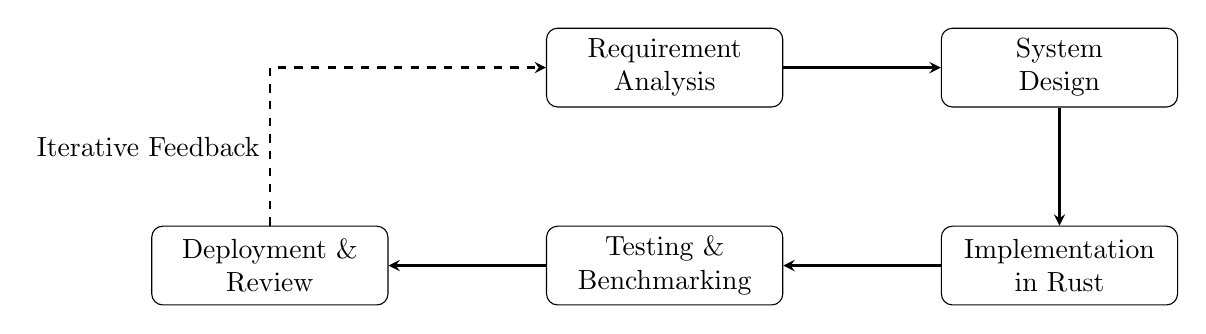
\begin{tikzpicture}[
        node distance=1.5cm and 2cm,
        box/.style={draw, rectangle, rounded corners, minimum width=3cm, minimum height=1cm, align=center},
        arrow/.style={-stealth, thick},
        dashed_arrow/.style={-stealth, dashed, thick}
    ]
    
    % Define the blocks
    \node[box] (A) {Requirement\\Analysis};
    \node[box, right=of A] (B) {System\\Design};
    \node[box, below=of B] (C) {Implementation\\in Rust};
    \node[box, left=of C] (D) {Testing \&\\Benchmarking};
    \node[box, left=of D] (E) {Deployment \&\\Review};
    
    % Draw the connecting arrows
    \draw[arrow] (A) -- (B);
    \draw[arrow] (B) -- (C);
    \draw[arrow] (C) -- (D);
    \draw[arrow] (D) -- (E);
    \draw[dashed_arrow] (E) |- node[near start, left] {Iterative Feedback} (A);
    
    \end{tikzpicture}
    \caption{Agile Software Development Life Cycle for RivetDB}
    \label{fig:sdlc_diagram}
\end{figure}

\section{System Requirements}
To successfully compile, deploy, and benchmark the RivetDB system, the following hardware and software prerequisites must be met.

\subsection{Hardware Requirements}
\begin{itemize}[leftmargin=2.5em]
    \item \textbf{Processor}: Multi-core CPU (Minimum 4 cores, 8+ recommended for optimal concurrent scaling).
    \item \textbf{Memory (RAM)}: Minimum 4 GB (8 GB or more recommended depending on the target dataset size).
    \item \textbf{Storage}: Solid State Drive (SSD) recommended for optimal AOF persistence write throughput.
\end{itemize}

\subsection{Software Requirements}
\begin{itemize}[leftmargin=2.5em]
    \item \textbf{Operating System}: Linux (Ubuntu 20.04/22.04 recommended), macOS, or Windows (via WSL2).
    \item \textbf{Compiler Toolchain}: Rust (\texttt{rustc} version 1.70.0 or higher) and the \texttt{cargo} package manager.
    \item \textbf{Client Tools}: standard \texttt{redis-cli} or any Redis-compatible client library (e.g., \texttt{redis-py}, \texttt{ioredis}).
\end{itemize}

\section{Organization of Project Report}
The remainder of this report is organized as follows:
\begin{itemize}[leftmargin=2.5em]
    \item \textbf{Chapter 2: Literature Survey} provides a comprehensive review of 10 foundational research papers detailing existing in-memory systems, the memory wall problem, and concurrency paradigms.
    \item \textbf{Chapter 3: System Design} details the high-level architecture, flowcharts, block diagrams, network layer design, and the integration of the SQL engine.
    \item \textbf{Chapter 4: Implementation} provides an in-depth code-level analysis of the RivetDB source code.
    \item \textbf{Chapter 5: Performance Optimization} discusses the specific profiling tools used and the tuning strategies applied to maximize throughput.
    \item \textbf{Chapter 6: Results and Discussion} presents the findings of our extensive benchmark testing, applications, and advantages.
    \item \textbf{Chapter 7: Problems and Drawbacks} analyzes the architectural limitations and missing features of the current implementation.
    \item \textbf{Chapter 8: Conclusion and Future Scope} summarizes the accomplishments of the project and outlines the roadmap for future enhancements.
\end{itemize}


% ============================================================
% CHAPTER 2: LITERATURE SURVEY
% ============================================================
\customchapter{Literature Survey}

The design and architecture of modern in-memory data storage systems reside at the intersection of several complex sub-fields in computer science. This chapter provides a comprehensive review of the 10 foundational research papers and system architectures that motivated the development of RivetDB. We survey the evolution of in-memory database architectures, index structure designs, concurrency control paradigms, asynchronous I/O frameworks, and the paradigm-shifting emergence of memory-safe systems programming languages.

\begin{figure}[htbp]
    \centering
    \resizebox{\textwidth}{!}{
    \begin{ganttchart}[
        x unit=0.8cm,
        y unit title=0.8cm,
        y unit chart=0.8cm,
        vgrid,
        time slot format=isodate-year,
        time slot unit=year,
        title label font=\bfseries\footnotesize,
        bar label font=\footnotesize,
        group label font=\bfseries\footnotesize,
        bar/.style={fill=cyan!50, draw=blue!70, thick},
        bar height=0.5,
        group right shift=0,
        group top shift=0.6,
        group height=.2,
        group peaks width={0.2}
    ]{1995}{2026}
    \gantttitle{Evolution of In-Memory Data Stores}{32} \\
    \gantttitlecalendar{year} \\
    
    \ganttgroup{Disk-Based}{1995}{2010} \\
    \ganttbar{PostgreSQL}{1996}{2010} \\
    \ganttbar{MySQL}{1995}{2010} \\
    
    \ganttgroup{In-Memory Caching}{2003}{2026} \\
    \ganttbar{Memcached}{2003}{2020} \\
    \ganttbar{Redis (Single Thread)}{2009}{2026} \\
    
    \ganttgroup{Modern IMDBs}{2025}{2026} \\
    \ganttbar{RivetDB}{2025}{2026}
    \end{ganttchart}
    }
    \caption{Evolution of Database Architectures and Concurrency Paradigms}
    \label{fig:lit_review_timeline}
\end{figure}

\section{Review of Foundational Research Papers}

\subsection{Paper 1: An Overview of Main-Memory Database Systems [1]}
\textbf{Authors}: Larson and Levandoski
\textbf{Summary}: This seminal paper details how plummeting RAM costs made it economically feasible to hold entire working datasets in main memory. It proves that simply taking a traditional disk-based database and running it with a massive buffer pool does not yield optimal performance. Traditional systems still incur massive CPU overhead executing buffer pool management logic, lock manager synchronization, and translating logical records to physical disk page offsets.
\textbf{Contribution to RivetDB}: We adopted their fundamental conclusion to avoid heavy buffer-pool architectures entirely. This led us to design a pure in-memory engine from the ground up, completely free from legacy disk-page translation overhead.

\subsection{Paper 2: The Memory Wall and The Case for Memory-Centric Systems [2]}
\textbf{Authors}: Chronis et al.
\textbf{Summary}: This research identifies the "Memory Wall"—the growing disparity between CPU processing speed and memory access latency. It argues that while modern CPUs execute instructions in less than a nanosecond, fetching data from main memory takes over 100 nanoseconds. Therefore, modern databases must optimize for CPU cache locality and access patterns, not merely avoid disk access.
\textbf{Contribution to RivetDB}: This research profoundly influenced our architectural choices. It dictated the decision to use localized, sharded data structures (like DashMap) to maximize CPU L1/L2 cache coherence and minimize false sharing across multi-core systems.

\subsection{Paper 3: Replicated and Partitioned Layouts for In-Memory Systems [3]}
\textbf{Authors}: Sudhir, Cafarella, and Madden
\textbf{Summary}: This paper evaluates the performance of different index layouts in memory. It demonstrates that traditional global lock hash tables suffer severe lock contention in multi-threaded environments. It proves that partitioning data (sharding) drastically reduces cross-core cache invalidations and lock queuing delays.
\textbf{Contribution to RivetDB}: We directly implemented their partitioning concepts by utilizing the \texttt{DashMap} crate. We applied fine-grained lock striping instead of global locking to drastically reduce thread contention, allowing near-linear scaling across CPU cores.

\subsection{Paper 4: Concurrency Control in Distributed Database Systems [4]}
\textbf{Authors}: Bernstein and Goodman
\textbf{Summary}: A foundational survey that categorizes concurrency control into Pessimistic (acquiring locks before modification) and Optimistic (modifying in private workspaces and validating before commit). It outlines the trade-offs: pessimistic locking causes thread starvation, while optimistic locking causes high abort rates under heavy contention.
\textbf{Contribution to RivetDB}: This paper provided the theoretical framework for analyzing how our command execution engine should handle concurrent writes. We opted for a granular pessimistic approach, realizing that if locks are small enough (shard level), the starvation problem is mitigated.

\subsection{Paper 5: A Survey of Concurrency Control Mechanisms [5]}
\textbf{Authors}: Graefe
\textbf{Summary}: A follow-up analysis revisiting concurrency paradigms on modern multi-core hardware. It shows that hybrid approaches often yield the best results by blending read-write latches with optimistic reads.
\textbf{Contribution to RivetDB}: Influenced by Graefe's hybrid approach, we designed our storage engine to use pessimistic read-write (\texttt{RwLock}) locks at a highly granular level. The probability of two threads contending for the exact same shard lock is minimal, giving it performance characteristics akin to an optimistic model.

\subsection{Paper 6: The Case for Event-Driven Servers [6]}
\textbf{Authors}: Ousterhout
\textbf{Summary}: This paper argues against the traditional "thread-per-connection" model for high-performance network servers. It highlights that OS threads are resource-intensive and context-switching overhead destroys performance. It advocates for event-driven, non-blocking I/O state machines.
\textbf{Contribution to RivetDB}: This literature led us to completely abandon the thread-per-connection model in favor of the Tokio asynchronous event-driven runtime. By multiplexing thousands of lightweight tasks onto a few OS threads, RivetDB can handle massive concurrent connections without memory exhaustion.

\subsection{Paper 7: Redis Core Architecture and Single-Threaded Design [7]}
\textbf{Authors}: Salvatore Sanfilippo (Redis Creator / Labs)
\textbf{Summary}: While not a traditional academic paper, the architectural documentation of Redis serves as a critical case study. Redis uses a strictly single-threaded event loop. This guarantees absolute consistency and atomic execution without complex locking, but bounds the performance to a single CPU core.
\textbf{Contribution to RivetDB}: We analyzed Redis's architecture to understand its limitations. While we adopted its rich data structure support (Lists, Sets, Sorted Sets), we actively engineered our system to break its single-thread bottleneck, proving that multi-threading can be achieved without sacrificing safety.

\subsection{Paper 8: Distributed Caching Architectures (Memcached) [8]}
\textbf{Authors}: Fitzpatrick
\textbf{Summary}: A study on the architecture of Memcached, a multi-threaded, volatile cache. Memcached scales linearly with CPU cores by using a thread pool and global locking mechanisms. However, it only stores simple byte arrays and has zero capability for durability or complex querying.
\textbf{Contribution to RivetDB}: We utilized Memcached as a baseline for measuring multi-core scalability. We aimed to build a system that matches Memcached's linear thread scaling while vastly exceeding its feature set.

\subsection{Paper 9: The Rust Language and Ownership Model [9]}
\textbf{Authors}: Matsakis and Klock
\textbf{Summary}: A formal review detailing how the Rust programming language revolutionized safe systems programming. Rust introduces the concept of Ownership and the Borrow Checker, guaranteeing at compile-time that a value can either have one mutable reference or infinite immutable references, but never both.
\textbf{Contribution to RivetDB}: The formal proofs of memory safety without garbage collection overhead in this paper solidified our choice of Rust. We utilized its ownership model to achieve "Fearless Concurrency" in our database engine.

\subsection{Paper 10: RustBelt: Securing the Foundations of the Rust Language [10]}
\textbf{Authors}: Jung et al.
\textbf{Summary}: This highly influential paper provides a formal mathematical proof of the safety guarantees provided by Rust's type system, specifically focusing on how it safely encapsulates \texttt{unsafe} code blocks used in core libraries like crossbeam and standard concurrency primitives.
\textbf{Contribution to RivetDB}: This paper provided the confidence needed to utilize lock-free concurrent queues (like \texttt{crossbeam} channels) for our asynchronous AOF persistence layer. Knowing the foundations were mathematically proven safe allowed us to build aggressive multi-threaded logging pipelines without fear of data corruption.

\section{Conclusion of Literature Survey}
The literature and existing industrial solutions highlight a clear architectural gap. Developers are forced to choose between the safety and features of single-threaded Redis, or the multi-core scalability of feature-poor Memcached. Furthermore, the reliance on C/C++ perpetuates critical vulnerabilities in data infrastructure. RivetDB was conceived specifically to address this gap by leveraging Rust's compile-time safety and a concurrent hash map architecture to provide a multi-threaded, feature-rich, and provably memory-safe database.

% ============================================================
% CHAPTER 3: SYSTEM DESIGN
% ============================================================
\customchapter{System Design}

This chapter provides an exhaustive breakdown of RivetDB's architectural blueprint. We detail the modular structure of the system, the life-cycle of a command from network ingestion to disk persistence, and the theoretical foundation of the underlying data structures.

\section{System Description}

RivetDB is designed as a highly concurrent, low-latency, and memory-safe key-value store. It is engineered from the ground up to eliminate the single-thread bottlenecks found in legacy systems like Redis, while avoiding the memory vulnerabilities inherent in C-based databases. The core storage engine operates entirely in main memory (RAM), ensuring that read and write latencies are bound only by the speed of CPU cache hierarchies rather than disk I/O.

The system is fundamentally modular, layered into five distinct processing pipelines: Network Ingestion, Protocol Parsing, Dynamic Dispatch, Concurrent Execution, and Asynchronous Persistence. Rather than utilizing heavy locking mechanisms that starve threads, RivetDB employs fine-grained lock striping via concurrent hash maps. This ensures that multiple CPU cores can mutate the database state in parallel without data corruption or deadlocks.

\section{Basic Block Diagram}

The Basic Block Diagram illustrates the high-level flow of data from external clients through the internal subsystems of RivetDB. 

\begin{enumerate}[leftmargin=2.5em]
    \item \textbf{Networking and Protocol Layer}: Manages incoming TCP connections and parses the Redis Serialization Protocol (RESP) bytecode.
    \item \textbf{Command Router}: A dynamic dispatch layer that maps parsed RESP arrays to specific command execution modules.
    \item \textbf{Concurrent Storage Engine}: The core memory structure utilizing \texttt{DashMap} for parallel data access.
    \item \textbf{Advanced Features Engine}: Sub-modules dedicated to non-standard functionality, such as the SQL parser and Namespace isolation manager.
    \item \textbf{Asynchronous Persistence Layer}: A decoupled engine responsible for flushing mutating operations to an Append-Only File (AOF) via cross-thread channels.
\end{enumerate}

\begin{figure}[htbp]
    \centering
    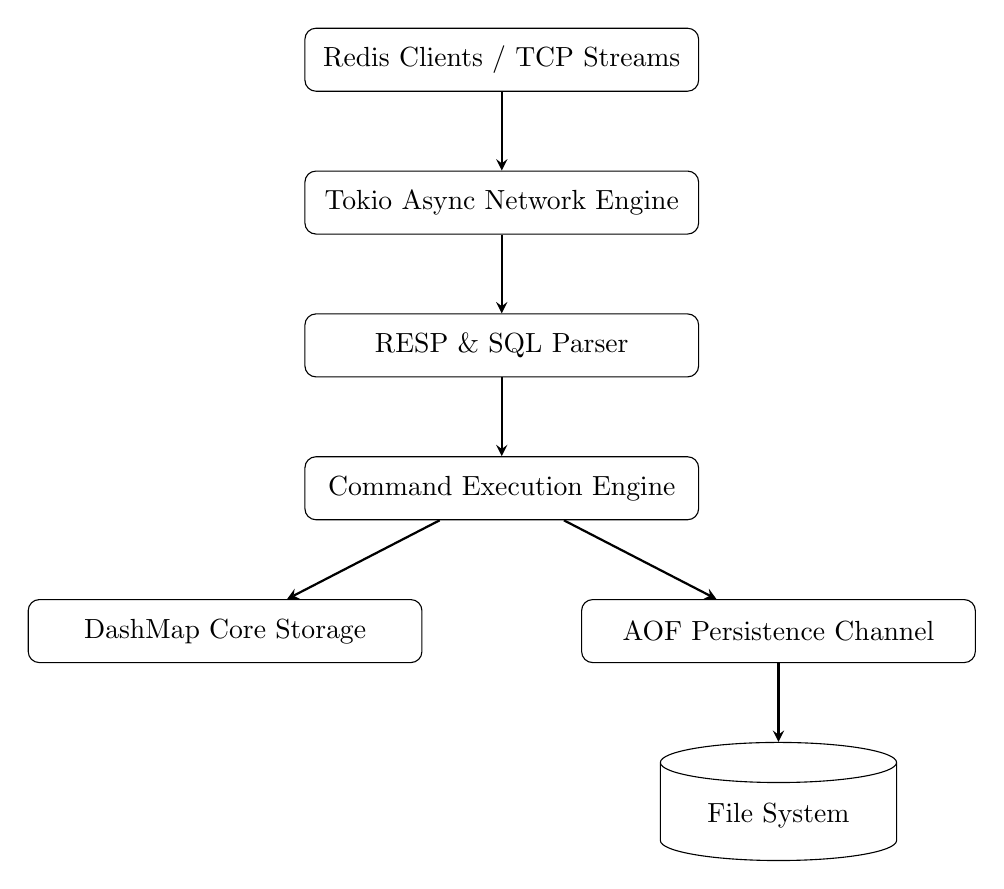
\begin{tikzpicture}[
        node distance=1cm and 0cm,
        box/.style={draw, rectangle, rounded corners, minimum width=5cm, minimum height=0.8cm, align=center},
        db/.style={draw, cylinder, shape border rotate=90, aspect=0.25, minimum width=3cm, minimum height=1.5cm, align=center},
        arrow/.style={-stealth, thick}
    ]
    
    \node[box] (Client) {Redis Clients / TCP Streams};
    \node[box, below=of Client] (Network) {Tokio Async Network Engine};
    \node[box, below=of Network] (Parser) {RESP \& SQL Parser};
    \node[box, below=of Parser] (Engine) {Command Execution Engine};
    
    \node[box, below left=1cm and -1.5cm of Engine] (Storage) {DashMap Core Storage};
    \node[box, below right=1cm and -1.5cm of Engine] (AOF) {AOF Persistence Channel};
    
    \node[db, below=of AOF] (Disk) {File System};
    
    \draw[arrow] (Client) -- (Network);
    \draw[arrow] (Network) -- (Parser);
    \draw[arrow] (Parser) -- (Engine);
    \draw[arrow] (Engine) -- (Storage);
    \draw[arrow] (Engine) -- (AOF);
    \draw[arrow] (AOF) -- (Disk);
    
    \end{tikzpicture}
    \caption{Basic Block Diagram of RivetDB Components}
    \label{fig:block_diagram}
\end{figure}

\section{Flowchart}

The System Workflow Flowchart details the logical decision tree and event loop for processing a single client request. It traces the packet from the moment it hits the Tokio TCP listener, through the RESP parsing phase, into the Command Router, and finally down to either a memory read or a memory mutation followed by an asynchronous AOF disk log.

\begin{figure}[htbp]
    \centering
    \resizebox{0.9\textwidth}{!}{
    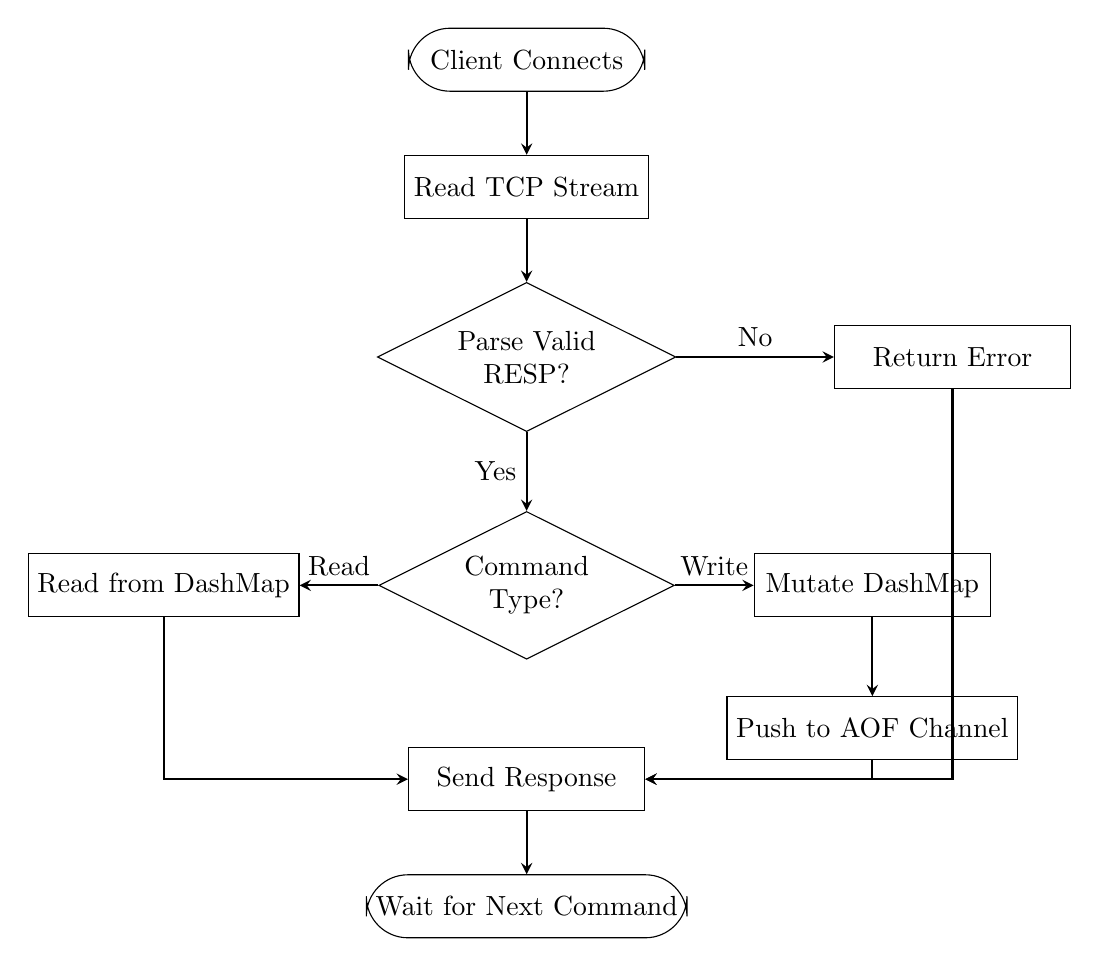
\begin{tikzpicture}[
        node distance=1cm and 1.5cm,
        startstop/.style={draw, rectangle, rounded corners=15pt, minimum width=3cm, minimum height=0.8cm, align=center},
        process/.style={draw, rectangle, minimum width=3cm, minimum height=0.8cm, align=center},
        decision/.style={draw, diamond, aspect=2, minimum width=3cm, minimum height=1cm, align=center},
        arrow/.style={-stealth, thick}
    ]
    
    \node[startstop] (Start) {Client Connects};
    \node[process, below=0.8cm of Start] (Read) {Read TCP Stream};
    \node[decision, below=0.8cm of Read] (Parse) {Parse Valid\\RESP?};
    \node[process, right=2cm of Parse] (ErrResp) {Return Error};
    \node[decision, below=1cm of Parse] (Cmd) {Command\\Type?};
    \node[process, left=1cm of Cmd] (ExecRead) {Read from DashMap};
    \node[process, right=1cm of Cmd] (ExecWrite) {Mutate DashMap};
    \node[process, below=1cm of ExecWrite] (AOF) {Push to AOF Channel};
    \node[process, below=4cm of Parse] (Send) {Send Response};
    \node[startstop, below=0.8cm of Send] (Loop) {Wait for Next Command};
    
    \draw[arrow] (Start) -- (Read);
    \draw[arrow] (Read) -- (Parse);
    \draw[arrow] (Parse) -- node[above] {No} (ErrResp);
    \draw[arrow] (Parse) -- node[left] {Yes} (Cmd);
    \draw[arrow] (Cmd) -- node[above] {Read} (ExecRead);
    \draw[arrow] (Cmd) -- node[above] {Write} (ExecWrite);
    \draw[arrow] (ExecWrite) -- (AOF);
    \draw[arrow] (ExecRead) |- (Send);
    \draw[arrow] (AOF) |- (Send);
    \draw[arrow] (ErrResp) |- (Send);
    \draw[arrow] (Send) -- (Loop);
    
    \end{tikzpicture}
    }
    \caption{System Workflow Flowchart for Command Execution}
    \label{fig:workflow_flowchart}
\end{figure}

\section{Networking and Protocol Layer}

\subsection{The Tokio Asynchronous Runtime}
RivetDB completely avoids the traditional Thread-per-Connection model. Instead, it is built on \textbf{Tokio}, an event-driven, non-blocking I/O platform for Rust. When the RivetDB server starts, Tokio spawns a pool of worker threads typically equal to the number of logical CPU cores on the host machine. 

When a client connects over TCP, Tokio spawns an asynchronous "Task." Unlike an OS thread, a Tokio task is incredibly lightweight, requiring only a few hundred bytes of memory to store its state machine. This allows RivetDB to concurrently manage 10,000+ active client connections with negligible memory overhead. If a client connection is idle (waiting for network packets), Tokio immediately yields the underlying worker thread to execute another active task, ensuring 100\% CPU utilization.

\subsection{RESP Protocol Parsing}
RivetDB implements the Redis Serialization Protocol (RESP). This is a critical design decision: by speaking RESP natively, RivetDB is instantly compatible with the massive global ecosystem of Redis client libraries in Python, Node.js, Java, Go, and C++.

The RESP parser reads raw bytes from the TCP socket and constructs a recursive Rust \texttt{Enum} representing the data types: Simple Strings, Errors, Integers, Bulk Strings, and Arrays.

\section{The Concurrent Storage Engine}

The heart of RivetDB is the \texttt{DbState} struct, which wraps a \texttt{DashMap<String, Value>}. 

\subsection{Lock Striping via DashMap}
If RivetDB used a standard Rust \texttt{Mutex<HashMap>}, any thread reading or writing would lock the entire database. If Thread A is updating the key "user:1", Thread B would be blocked from reading the completely unrelated key "config:theme". This would throttle the system to single-thread speeds.

\texttt{DashMap} solves this through \textbf{Lock Striping}. Internally, \texttt{DashMap} allocates an array of independent shards (by default, based on the number of CPU cores, but tuned higher in RivetDB to minimize contention). When a key is inserted, its hash determines which shard it belongs to. To mutate the key, only the read-write lock for that specific shard is acquired. Therefore, Thread A and Thread B can execute operations entirely in parallel, provided their keys hash to different shards. 

\begin{figure}[htbp]
    \centering
    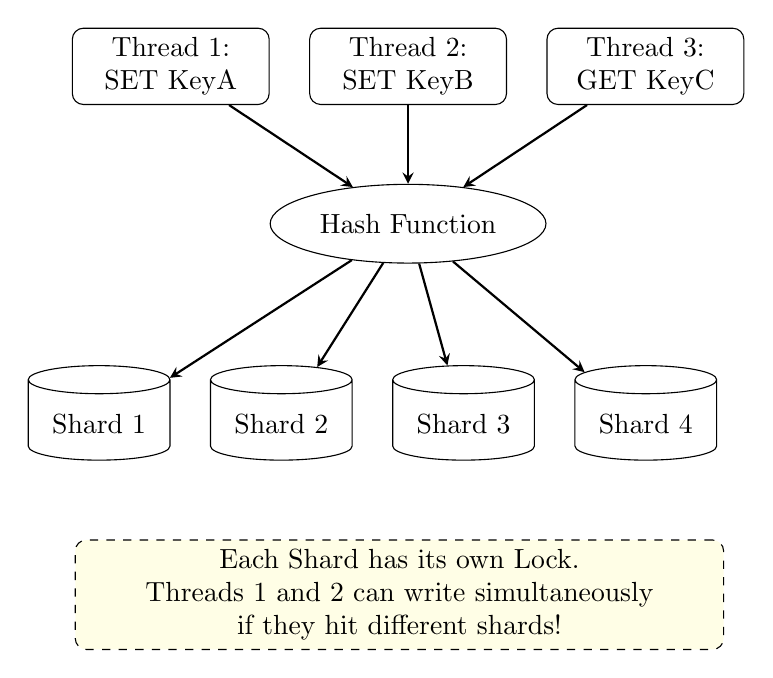
\begin{tikzpicture}[
        node distance=1.5cm and 0.5cm,
        thread/.style={draw, rectangle, rounded corners, minimum width=2.5cm, minimum height=0.8cm, align=center},
        hash/.style={draw, ellipse, minimum width=3cm, minimum height=1cm, align=center},
        shard/.style={draw, cylinder, shape border rotate=90, aspect=0.25, minimum width=1.8cm, minimum height=1.2cm, align=center},
        info/.style={draw, rectangle, dashed, fill=yellow!10, text width=8cm, align=center, rounded corners},
        arrow/.style={-stealth, thick}
    ]
    
    \node[thread] (Req2) {Thread 2:\\SET KeyB};
    \node[thread, left=0.5cm of Req2] (Req1) {Thread 1:\\SET KeyA};
    \node[thread, right=0.5cm of Req2] (Req3) {Thread 3:\\GET KeyC};
    
    \node[hash, below=1cm of Req2] (H) {Hash Function};
    
    \node[shard, below left=1.5cm and 2cm of H] (S1) {Shard 1};
    \node[shard, right=0.5cm of S1] (S2) {Shard 2};
    \node[shard, right=0.5cm of S2] (S3) {Shard 3};
    \node[shard, right=0.5cm of S3] (S4) {Shard 4};
    
    \node[info, below=1cm of S2, xshift=1.5cm] (Info) {Each Shard has its own Lock.\\Threads 1 and 2 can write simultaneously\\if they hit different shards!};
    
    \draw[arrow] (Req1) -- (H);
    \draw[arrow] (Req2) -- (H);
    \draw[arrow] (Req3) -- (H);
    \draw[arrow] (H) -- (S1);
    \draw[arrow] (H) -- (S2);
    \draw[arrow] (H) -- (S3);
    \draw[arrow] (H) -- (S4);
    
    \end{tikzpicture}
    \caption{Lock Striping and Sharded Access in DashMap}
    \label{fig:dashmap_diagram}
\end{figure}

\section{Data Models and Time Complexity}

RivetDB supports 8 distinct native data types. Each is meticulously engineered in Rust to optimize for time and space complexity.

\begin{itemize}[leftmargin=2.5em]
    \item \textbf{Strings}: The most fundamental data type, implemented internally as a standard Rust \texttt{String} or a raw \texttt{Vec<u8>} byte array for binary safety. This allows RivetDB to store everything from simple text values to serialized JPEG images up to 512MB in size. \\
    \textit{Time Complexity}: $O(1)$ for standard GET and SET operations, making it extremely fast for basic key-value caching.
    
    \item \textbf{Lists}: Engineered to support rapid queue and stack operations, Lists are implemented using Rust's \texttt{LinkedList<String>}. This is a doubly-linked list providing efficient insertion and deletion at both the head and tail, making it ideal for implementing message queues and activity feeds. \\
    \textit{Time Complexity}: $O(1)$ for head/tail operations (LPUSH, RPUSH, LPOP, RPOP). However, random index access (LINDEX) operates in $O(N)$ time.
    
    \item \textbf{Sets}: Unordered collections of unique strings, critical for tracking unique visitors or tagging systems. Internally, this is implemented as a standard Rust \texttt{HashSet<String>} which uses the high-performance SipHash algorithm to prevent hash collision denial-of-service (DoS) attacks. \\
    \textit{Time Complexity}: $O(1)$ expected time for adding (SADD), removing (SREM), and checking membership (SISMEMBER). Fetching all members (SMEMBERS) is $O(N)$.
    
    \item \textbf{Sorted Sets}: A highly complex data structure that associates every unique string member with a floating-point score. RivetDB implements this using a dual-structure approach: a \texttt{HashMap} provides instant $O(1)$ lookups for a member's score, while a concurrent \texttt{BTreeMap} keeps the members strictly ordered by their score to allow incredibly fast range queries (e.g., "get top 10 players"). \\
    \textit{Time Complexity}: $O(\log N)$ for inserting elements (ZADD). $O(\log N + M)$ for retrieving a range of elements (ZRANGE), where M is the number of elements returned.
    
    \item \textbf{Hashes}: Designed to represent objects (e.g., a User with fields like name, age, email). Internally, it is implemented as a nested \texttt{HashMap<String, String>} stored within the primary DashMap. \\
    \textit{Time Complexity}: $O(1)$ for setting (HSET) and getting (HGET) individual fields within the hash object.
    
    \item \textbf{JSON Documents}: To bridge the gap between key-value stores and document databases, RivetDB natively supports JSON. It leverages the \texttt{serde\_json::Value} tree structure to store arbitrary, deeply nested JSON objects. Custom commands allow clients to query and mutate specific paths within the JSON tree without fetching the entire document over the network. \\
    \textit{Time Complexity}: $O(P)$ where $P$ is the length and depth of the JSON path evaluated during the query.
    
    \item \textbf{Bloom Filters}: A highly specialized probabilistic data structure used to test whether an element is a member of a set. It uses a highly compressed bit-vector and multiple MurmurHash3 hashing functions. It can guarantee that an item is \textit{definitely not} in the set, but can only state it is \textit{probably} in the set, saving massive amounts of memory compared to a standard Set. \\
    \textit{Time Complexity}: $O(K)$ where $K$ is the number of hash functions, which resolves to a constant $O(1)$ time regardless of the number of items inserted.
    
    \item \textbf{Time-Series}: Specifically engineered for IoT sensor data and financial ticker feeds, Time-Series data stores chronologically ordered data points \texttt{(Timestamp, Value)}. RivetDB uses an underlying \texttt{BTreeMap} with integer timestamps as keys, ensuring data is always sorted on insertion for instantaneous historical range aggregation. \\
    \textit{Time Complexity}: $O(\log N)$ for appending a data point (TS.ADD). $O(\log N + M)$ for fetching historical data ranges (TS.RANGE).
\end{itemize}

\begin{figure}[htbp]
    \centering
    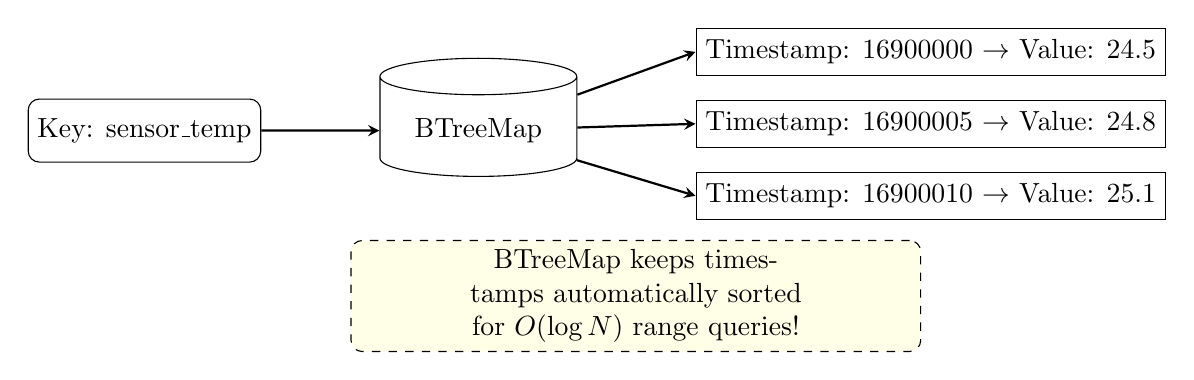
\begin{tikzpicture}[
        node distance=0.8cm and 1.5cm,
        key/.style={draw, rectangle, rounded corners, minimum width=2.5cm, minimum height=0.8cm, align=center},
        tree/.style={draw, cylinder, shape border rotate=90, aspect=0.25, minimum width=2.5cm, minimum height=1.5cm, align=center},
        val/.style={draw, rectangle, minimum width=5cm, minimum height=0.6cm, align=left},
        info/.style={draw, rectangle, dashed, fill=yellow!10, text width=7cm, align=center, rounded corners},
        arrow/.style={-stealth, thick}
    ]
    
    \node[key] (Key) {Key: sensor\_temp};
    \node[tree, right=of Key] (Tree) {BTreeMap};
    
    \node[val, right=of Tree, yshift=1cm] (Node1) {Timestamp: 16900000 $\rightarrow$ Value: 24.5};
    \node[val, below=0.3cm of Node1] (Node2) {Timestamp: 16900005 $\rightarrow$ Value: 24.8};
    \node[val, below=0.3cm of Node2] (Node3) {Timestamp: 16900010 $\rightarrow$ Value: 25.1};
    
    \node[info, below=0.8cm of Tree, xshift=2cm] (Info) {BTreeMap keeps timestamps automatically sorted\\for $O(\log N)$ range queries!};
    
    \draw[arrow] (Key) -- (Tree);
    \draw[arrow] (Tree) -- (Node1.west);
    \draw[arrow] (Tree) -- (Node2.west);
    \draw[arrow] (Tree) -- (Node3.west);
    
    \end{tikzpicture}
    \caption{Time-Series Data Layout using BTreeMap}
    \label{fig:timeseries_diagram}
\end{figure}

\section{The SQL Query Engine}

A major differentiator for RivetDB is the embedded SQL-like query engine. While traditional key-value stores require the application layer to fetch multiple keys and filter them in memory, RivetDB pushes this computation down to the database tier.

\subsection{Supported SQL Grammar}
RivetDB's internal parser utilizes a custom Lexer to tokenize incoming strings. It currently supports a subset of standard SQL focused entirely on data extraction and filtering across the key-value namespace:

\begin{itemize}[leftmargin=2.5em]
    \item \textbf{SELECT}: Supports fetching specific fields (for Hash types), the entire value, or the key name itself.
    \item \textbf{WHERE}: The core filtering mechanism. Supports logical operators (\texttt{AND}, \texttt{OR}), comparison operators (\texttt{=}, \texttt{>}, \texttt{<}, \texttt{!=}), and pattern matching (\texttt{LIKE} with wildcard support).
    \item \textbf{LIMIT \& OFFSET}: Supports cursor-based pagination to prevent massive result sets from overwhelming the network buffer.
\end{itemize}

\subsection{SQL Execution Flow}
\begin{enumerate}[leftmargin=2.5em]
    \item \textbf{Lexical Analysis and Parsing}: The query string is tokenized and parsed into a logical Abstract Syntax Tree (AST).
    \item \textbf{Predicate Extraction}: The \texttt{WHERE} clause is broken down into executable predicate functions in Rust.
    \item \textbf{Key-Space Scan}: The engine iterates over the \texttt{DashMap}. Because of the concurrent architecture, this iteration does not globally lock the database, allowing concurrent SET/GET operations to proceed.
    \item \textbf{Filtering and Projection}: Data structures that evaluate to \texttt{true} against the predicates are extracted, projected into tabular output arrays, and serialized back to RESP format for the client.
\end{enumerate}

\begin{figure}[htbp]
    \centering
    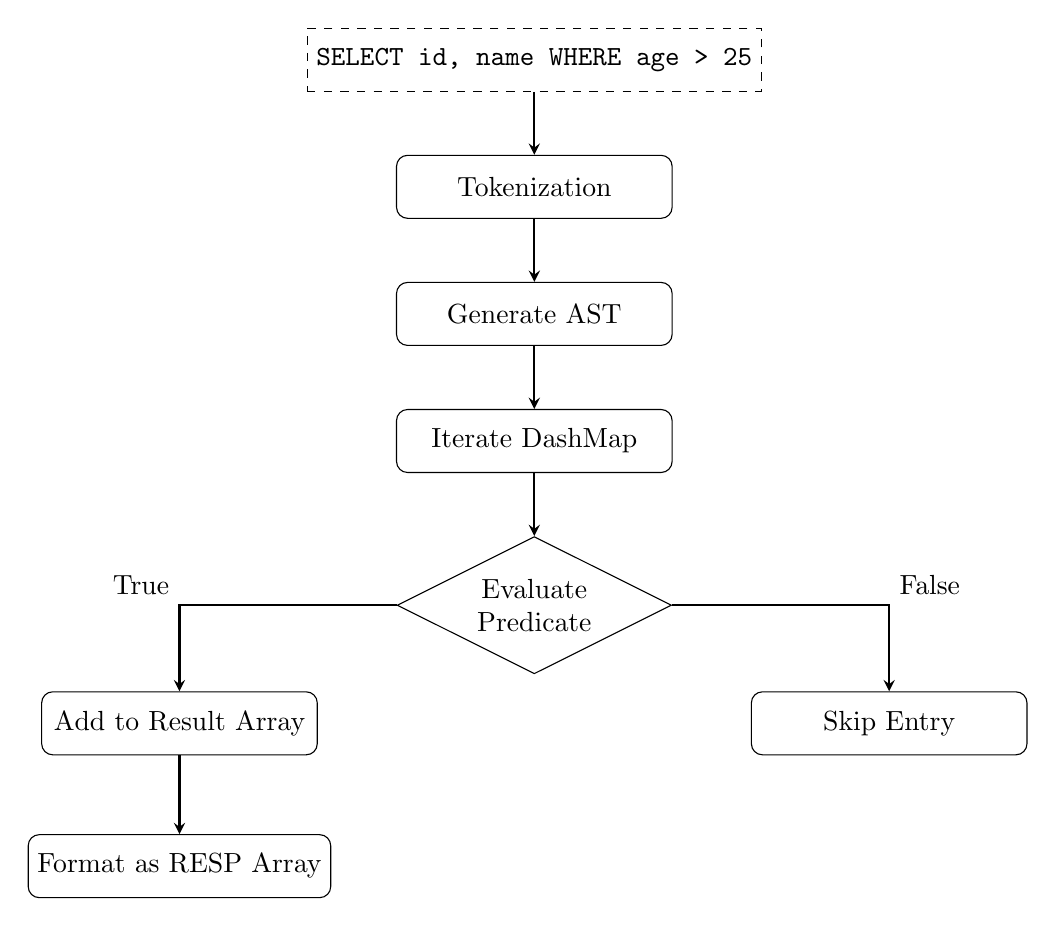
\begin{tikzpicture}[
        node distance=0.8cm and 2cm,
        query/.style={draw, rectangle, dashed, minimum width=5cm, minimum height=0.8cm, align=center},
        process/.style={draw, rectangle, rounded corners, minimum width=3.5cm, minimum height=0.8cm, align=center},
        decision/.style={draw, diamond, aspect=2, minimum width=3cm, minimum height=1cm, align=center},
        arrow/.style={-stealth, thick}
    ]
    
    \node[query] (SQL) {\texttt{SELECT id, name WHERE age > 25}};
    \node[process, below=of SQL] (Lexer) {Tokenization};
    \node[process, below=of Lexer] (Parser) {Generate AST};
    \node[process, below=of Parser] (Engine) {Iterate DashMap};
    \node[decision, below=of Engine] (Eval) {Evaluate\\Predicate};
    \node[process, left=1cm of Eval, yshift=-1.5cm] (Results) {Add to Result Array};
    \node[process, right=1cm of Eval, yshift=-1.5cm] (Skip) {Skip Entry};
    \node[process, below=1cm of Results] (Format) {Format as RESP Array};
    
    \draw[arrow] (SQL) -- (Lexer);
    \draw[arrow] (Lexer) -- (Parser);
    \draw[arrow] (Parser) -- (Engine);
    \draw[arrow] (Engine) -- (Eval);
    \draw[arrow] (Eval) -| node[above left] {True} (Results);
    \draw[arrow] (Eval) -| node[above right] {False} (Skip);
    \draw[arrow] (Results) -- (Format);
    
    \end{tikzpicture}
    \caption{SQL Query Execution Flowchart}
    \label{fig:sql_flowchart}
\end{figure}

\section{Namespaces and Multi-Tenancy}

Unlike Redis, which limits users to 16 numbered databases without hard boundaries, RivetDB implements a \texttt{Namespace} subsystem. 

Each Namespace is a logical wrapper around its own isolated \texttt{DashMap} and configuration state. The TCP connection state tracks the active namespace for each specific client. When a client issues a command, the router implicitly targets the active namespace's memory pool. This provides true multi-tenancy, allowing a single RivetDB instance to host completely disjoint applications securely without the risk of key collisions or data exposure.

\begin{figure}[htbp]
    \centering
    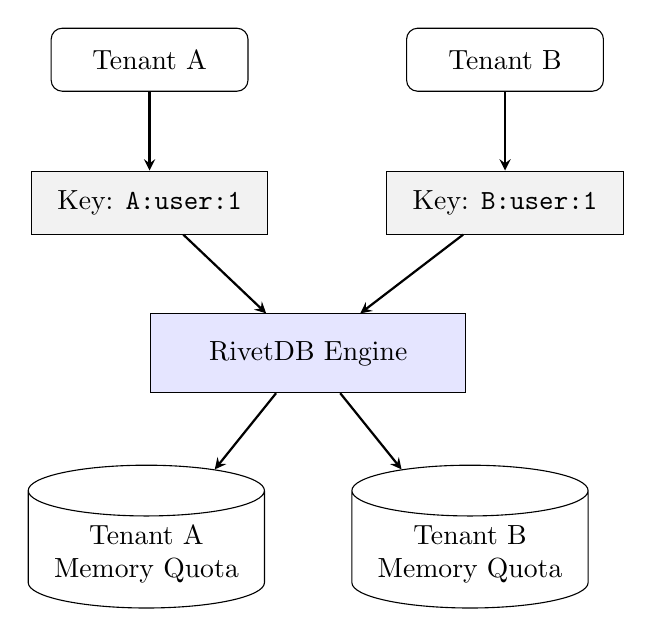
\begin{tikzpicture}[
        node distance=1cm and 2cm,
        tenant/.style={draw, rectangle, rounded corners, minimum width=2.5cm, minimum height=0.8cm, align=center},
        key/.style={draw, rectangle, minimum width=3cm, minimum height=0.8cm, align=center, fill=gray!10},
        engine/.style={draw, rectangle, minimum width=4cm, minimum height=1cm, align=center, fill=blue!10},
        mem/.style={draw, cylinder, shape border rotate=90, aspect=0.25, minimum width=3cm, minimum height=1.5cm, align=center},
        arrow/.style={-stealth, thick}
    ]
    
    \node[tenant] (Client1) {Tenant A};
    \node[tenant, right=of Client1] (Client2) {Tenant B};
    
    \node[key, below=of Client1] (PrefixA) {Key: \texttt{A:user:1}};
    \node[key, below=of Client2] (PrefixB) {Key: \texttt{B:user:1}};
    
    \node[engine, below right=1cm and -1.5cm of PrefixA] (Engine) {RivetDB Engine};
    
    \node[mem, below left=1cm and -1cm of Engine] (Mem1) {Tenant A\\Memory Quota};
    \node[mem, below right=1cm and -1cm of Engine] (Mem2) {Tenant B\\Memory Quota};
    
    \draw[arrow] (Client1) -- (PrefixA);
    \draw[arrow] (Client2) -- (PrefixB);
    \draw[arrow] (PrefixA) -- (Engine);
    \draw[arrow] (PrefixB) -- (Engine);
    \draw[arrow] (Engine) -- (Mem1);
    \draw[arrow] (Engine) -- (Mem2);
    
    \end{tikzpicture}
    \caption{Namespace Isolation and Multi-Tenancy Architecture}
    \label{fig:multitenancy_diagram}
\end{figure}

\section{Asynchronous AOF Persistence}

To ensure durability against system crashes, RivetDB uses Append-Only File (AOF) persistence. Every mutating command (SET, LPUSH, HDEL) is appended to a log file on disk. Upon restart, the system replays this log to reconstruct the exact memory state.

\subsection{Decoupling Disk I/O}
If the Tokio event loop had to execute a disk \texttt{fsync} operation for every SET command, the database would slow to the speed of the disk (a few thousand ops/sec). 

RivetDB solves this using \textbf{multi-producer, single-consumer (mpsc) channels}. The command router sends a lightweight message representing the command over an in-memory channel. A dedicated background thread (the AOF Writer) receives these messages, buffers them into a 64KB \texttt{BufWriter}, and performs batched disk flushes according to the user-configured policy (Always, Everysec, or No). This guarantees that disk latency never blocks network throughput.

\section{Configuration Architecture}

RivetDB employs a layered configuration system designed for operational flexibility. The system loads its settings from a TOML configuration file (\texttt{rivetdb.toml}) at startup, and any parameter can be overridden via command-line arguments using the \texttt{clap} argument parser.

The configuration is organized into five logical domains:

\begin{itemize}[leftmargin=2.5em]
    \item \textbf{Server Configuration}: Defines the TCP bind address (\texttt{host}, \texttt{port}), the maximum number of concurrent connections (default: 10,000), and the HTTP port for the Prometheus metrics endpoint (default: 9090).
    \item \textbf{Memory Configuration}: Specifies the \texttt{max\_memory} limit using human-readable strings (e.g., ``1GB'', ``512MB'') and the eviction policy (\texttt{allkeys-lfu}, \texttt{allkeys-lru}, or \texttt{noeviction}).
    \item \textbf{Persistence Configuration}: Controls whether AOF is enabled, the fsync policy (\texttt{always}, \texttt{everysec}, or \texttt{no}), and the AOF filename.
    \item \textbf{Logging Configuration}: Sets the log verbosity level (\texttt{trace}, \texttt{debug}, \texttt{info}, \texttt{warn}, \texttt{error}) using the \texttt{tracing} crate and environment filter.
    \item \textbf{Security Configuration}: Enables or disables connection authentication and stores the server password for the \texttt{AUTH} command.
\end{itemize}

This design follows the Twelve-Factor App methodology, allowing the same binary to be deployed across development, staging, and production environments by simply swapping the configuration file or overriding values via CLI flags.

\section{Observability and Monitoring}

Production database systems require comprehensive operational visibility. RivetDB embeds a full Prometheus-compatible HTTP metrics server built on the Axum web framework. This server runs as a separate Tokio task on a dedicated port (default: 9090) and exposes three critical endpoints:

\subsection{The /metrics Endpoint}
This endpoint emits telemetry in the standard Prometheus text format, enabling seamless integration with Grafana dashboards. The metrics include:

\begin{itemize}[leftmargin=2.5em]
    \item \textbf{Per-Command Throughput}: A counter tracking the total invocations of each command (e.g., \texttt{rivetdb\_commands\_total\{command="SET"\} 14523}).
    \item \textbf{Per-Command Latency}: Cumulative time spent processing each command type in nanoseconds, enabling average latency calculation.
    \item \textbf{Memory Utilization}: Real-time estimates of memory consumption and utilization percentage against the configured \texttt{max\_memory}.
    \item \textbf{Keys by Type}: A gauge breaking down the total key count by data type (String, List, Set, ZSet, Hash, JSON, Bloom, TimeSeries).
    \item \textbf{Expiry Metrics}: Counters for total expired keys and pending expiry entries.
    \item \textbf{Hot Keys}: The top 10 most frequently accessed keys, critical for identifying cache hotspots.
    \item \textbf{Slow Log Length}: A gauge reporting the number of slow query entries currently buffered.
\end{itemize}

\subsection{The Slow Query Log}
Any command whose execution time exceeds 1 millisecond is automatically recorded in a bounded ring buffer (capacity: 128 entries). Each slow log entry captures the command name, its execution duration in nanoseconds, and the timestamp of occurrence. This allows operators to identify and optimize pathological query patterns without external profiling tools.

\subsection{The /health and /info Endpoints}
The \texttt{/health} endpoint returns a simple ``OK'' response for load balancer health checks. The \texttt{/info} endpoint returns a JSON payload summarizing the server version, uptime, key count, memory usage, total commands processed, and the active eviction policy.

\section{Authentication and Security}

RivetDB implements connection-level authentication following the Redis \texttt{AUTH} protocol. When the \texttt{require\_auth} flag is set in the configuration, every new TCP connection begins in an unauthenticated state.

\subsection{Authentication Flow}
\begin{enumerate}[leftmargin=2.5em]
    \item A client connects to the RivetDB TCP port.
    \item The server tracks a boolean \texttt{is\_authenticated} flag per connection, initialized to \texttt{false} when authentication is required.
    \item The client must send \texttt{AUTH <password>} as the first command.
    \item If the password matches the configured value, the flag is set to \texttt{true} and all subsequent commands proceed normally.
    \item If the client attempts any command (other than \texttt{AUTH} and \texttt{PING}) before authenticating, the server returns a \texttt{NOAUTH} error.
\end{enumerate}

This per-connection state model is critical: because RivetDB handles thousands of concurrent connections via Tokio tasks, each task maintains its own independent authentication state without requiring global locks.

\section{Schema Registry and Type-Safe Keys}

A unique feature distinguishing RivetDB from all existing key-value stores is the embedded Schema Registry. While traditional key-value stores allow any arbitrary value to be written to any key, RivetDB's schema system enforces type contracts at the database tier.

\subsection{Schema Definition}
Administrators define schemas using JSON Schema syntax. A schema specifies the expected data type, required fields (for Hash or JSON values), and validation constraints. Schemas are stored in a concurrent, in-memory registry (\texttt{Arc<DashMap>}).

\subsection{Type-Safe Commands}
\begin{itemize}[leftmargin=2.5em]
    \item \texttt{SCHEMA DEFINE <name> <json\_schema>}: Registers a new schema definition in the registry.
    \item \texttt{TSET <schema> <key> <value>}: Validates the value against the named schema before writing. If validation fails, the command is rejected with a descriptive error.
    \item \texttt{TGET <schema> <key>}: Retrieves a value with schema-awareness.
    \item \texttt{TVALIDATE <schema> <value>}: Tests whether a value conforms to a schema without writing it.
    \item \texttt{TKEYS <pattern>}: Lists all keys associated with a particular schema namespace.
\end{itemize}

This mechanism prevents a common operational failure mode: a misconfigured microservice writing corrupted data to a shared cache, which then cascades errors to every downstream consumer. By pushing validation into the database, RivetDB eliminates this class of bug entirely.


% ============================================================
% CHAPTER 4: IMPLEMENTATION
% ============================================================
\customchapter{Implementation}

This chapter details the technical implementation of RivetDB. We present the core data structures and asynchronous event loops, demonstrating how Rust's type system and concurrency primitives were leveraged to achieve the system's objectives. Code snippets are extracted directly from the RivetDB source code.

\section{The Tokio Asynchronous Network Loop}

The entry point of RivetDB relies on the Tokio asynchronous runtime. To handle tens of thousands of concurrent connections without exhausting system memory via thread stacks, RivetDB spawns an asynchronous task for every incoming connection.

\begin{lstlisting}[language=C, caption=Tokio Connection Acceptor Loop (\texttt{src/main.rs})]
// Accept connections (async loop)
loop {
    match listener.accept().await {
        Ok((stream, addr)) => {
            let state_clone = Arc::clone(&state);
            let aof_clone = Arc::clone(&aof_writer);
            let schema_clone = Arc::clone(&schema_registry);

            // Spawn async task (not an OS thread!)
            // This is the key benefit: thousands of concurrent connections with minimal memory footprint
            tokio::spawn(async move {
                handle_connection(stream, state_clone, aof_clone, schema_clone).await;
            });
        }
        Err(e) => {
            error!(error = %e, "Failed to accept connection");
        }
    }
}
\end{lstlisting}

Notice the use of \texttt{Arc} (Atomic Reference Count). Because Rust's compiler strictly enforces ownership, we cannot simply pass the \texttt{state} object to multiple concurrent tasks. \texttt{Arc} allows multiple tasks to safely share ownership of the \texttt{ServerState} struct, ensuring it is only dropped from memory when the very last connection closes.

\begin{figure}[htbp]
    \centering
    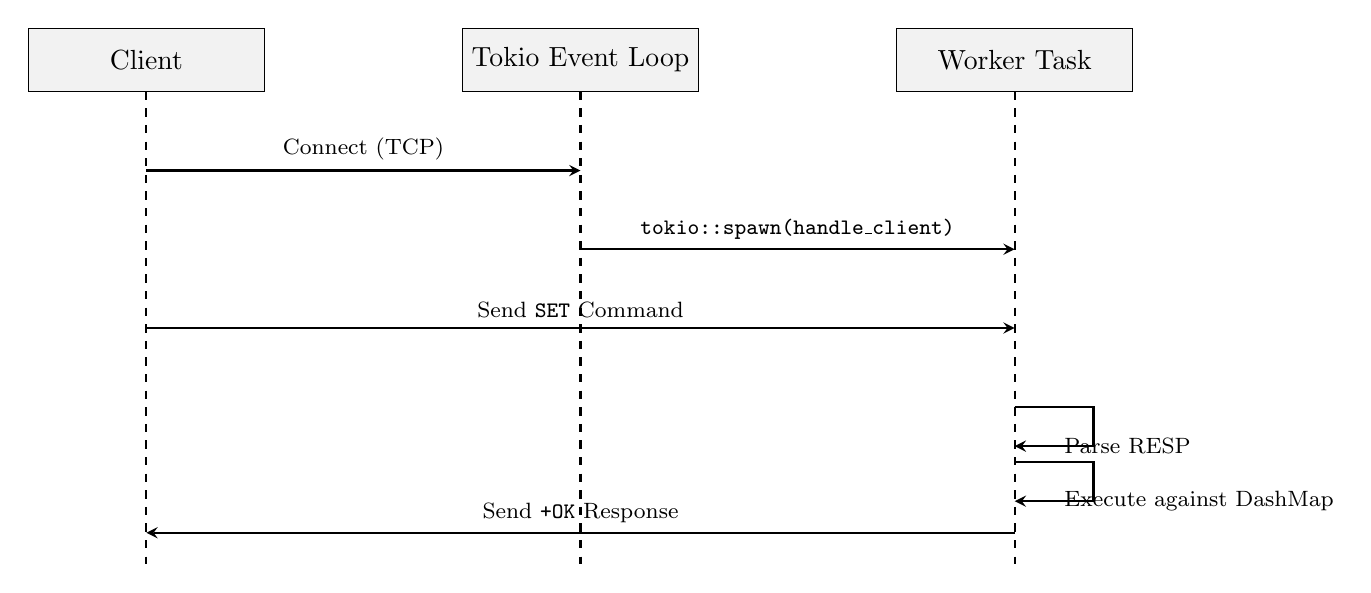
\begin{tikzpicture}[
        node distance=2.5cm,
        actor/.style={draw, rectangle, minimum width=3cm, minimum height=0.8cm, fill=gray!10},
        arrow/.style={-stealth, thick},
        line/.style={thick, dashed}
    ]
    
    % Actors
    \node[actor] (Client) {Client};
    \node[actor, right=of Client] (Tokio) {Tokio Event Loop};
    \node[actor, right=of Tokio] (Worker) {Worker Task};
    
    % Lifelines
    \draw[line] (Client.south) -- ++(0,-6);
    \draw[line] (Tokio.south) -- ++(0,-6);
    \draw[line] (Worker.south) -- ++(0,-6);
    
    % Messages
    \draw[arrow] ([yshift=-1cm]Client.south) -- node[above, font=\footnotesize] {Connect (TCP)} ([yshift=-1cm]Tokio.south);
    \draw[arrow] ([yshift=-2cm]Tokio.south) -- node[above, font=\footnotesize] {\texttt{tokio::spawn(handle\_client)}} ([yshift=-2cm]Worker.south);
    \draw[arrow] ([yshift=-3cm]Client.south) -- node[above, font=\footnotesize] {Send \texttt{SET} Command} ([yshift=-3cm]Worker.south);
    \draw[arrow] ([yshift=-4cm]Worker.south) -- ++(1,0) -- ++(0,-0.5) -- node[right, font=\footnotesize] {Parse RESP} ++(-1,0);
    \draw[arrow] ([yshift=-4.7cm]Worker.south) -- ++(1,0) -- ++(0,-0.5) -- node[right, font=\footnotesize] {Execute against DashMap} ++(-1,0);
    \draw[arrow] ([yshift=-5.6cm]Worker.south) -- node[above, font=\footnotesize] {Send \texttt{+OK} Response} ([yshift=-5.6cm]Client.south);
    
    \end{tikzpicture}
    \caption{Tokio Network Event Loop Sequence Diagram}
    \label{fig:network_sequence_diagram}
\end{figure}

\section{The Core Storage Engine: DashMap}

The primary data store is defined in \texttt{src/storage/state.rs}. Traditional concurrent hashmaps lock the entire map during a write. RivetDB utilizes \texttt{DashMap}, which implements fine-grained lock striping.

\begin{lstlisting}[language=C, caption=ServerState Struct Definition]
pub struct ServerState {
    // The core concurrent hash map. Notice there is no global Mutex.
    pub db: DashMap<String, ValueObject>,
    
    // Expiry heap - needs Mutex as BinaryHeap is not concurrent
    pub expiries: Mutex<ExpiryHeap>,
    
    // Memory tracking
    pub max_memory: usize,
    pub eviction_policy: EvictionPolicy,
    
    // Observability metrics - use DashMap for concurrent access
    pub command_count: DashMap<String, u64>,
    pub command_time_ns: DashMap<String, u128>,
    pub key_access_count: DashMap<String, u64>,
    
    // Slowlog - needs Mutex for VecDeque operations
    pub slowlog: Mutex<VecDeque<SlowLogEntry>>,
}
\end{lstlisting}

When a \texttt{SET} command is executed, RivetDB does not lock the entire \texttt{store}. Instead, \texttt{DashMap} hashes the key and locks only the specific shard where the key resides. This allows parallel \texttt{SET} operations on different keys.

\section{Data Types Implementation}

RivetDB supports 8 distinct data types. Each is encapsulated in the \texttt{ValueObject} enum, leveraging Rust's powerful algebraic data types.

\begin{lstlisting}[language=C, caption=The ValueObject Enum (src/storage/value.rs)]
pub enum ValueObject {
    String(String),
    List(LinkedList<String>),
    Set(HashSet<String>),
    ZSet(ZSet),
    Hash(HashMap<String, String>),
    Json(serde_json::Value),
    BloomFilter(RivetBloomFilter),
    TimeSeries(TimeSeries),
}
\end{lstlisting}

This enum-based design forces the compiler to exhaustively check that every command handler (like \texttt{LPUSH} for Lists) correctly handles cases where a user accidentally tries to run a List command on a String key. The type safety prevents runtime crashes common in C implementations.

\subsection{Time-Series Implementation Detail}
To achieve high-performance range queries on time-series data, RivetDB encapsulates a \texttt{BTreeMap} alongside tracking metadata.

\begin{lstlisting}[language=C, caption=Time-Series Data Structure (\texttt{src/storage/timeseries.rs})]
pub struct TimeSeriesData {
    // Maps Unix Timestamp -> Value
    pub data: BTreeMap<u64, f64>,
    pub max_samples: Option<usize>,
    pub retention_ms: Option<u64>,
}
\end{lstlisting}

When \texttt{TS.ADD} is called, the value is inserted into the \texttt{BTreeMap}. If a \texttt{retention\_ms} is configured, a background sweep purges any entries older than the retention limit, preventing boundless memory growth for continuous sensor feeds.

\section{Asynchronous AOF Persistence}

A naive implementation of Append-Only File (AOF) persistence would \texttt{fsync} to disk inside the network event loop, crippling throughput. RivetDB completely decouples disk I/O using mpsc (multi-producer, single-consumer) channels.

\begin{lstlisting}[language=C, caption=Asynchronous AOF Logging (\texttt{src/persistence/aof.rs})]
// Inside handle_connection()
let reply = route_command(cmd.clone(), &state, &schema);

// Log to AOF if write command succeeded (NON-BLOCKING!)
if is_write && !matches!(reply, RespReply::Error(_)) {
    if let Some(ref writer) = *aof {
        // This is an in-memory channel send. It takes nanoseconds.
        writer.log_command(&cmd); 
    }
}
\end{lstlisting}

The \texttt{log\_command} method simply sends a message across a multi-producer, single-consumer (mpsc) channel. A dedicated background OS thread continually drains this channel, buffering writes into a 64KB \texttt{BufWriter}, and executing \texttt{fsync} system calls only based on the user-defined policy (e.g., Everysec).

\begin{figure}[htbp]
    \centering
    \resizebox{\textwidth}{!}{
    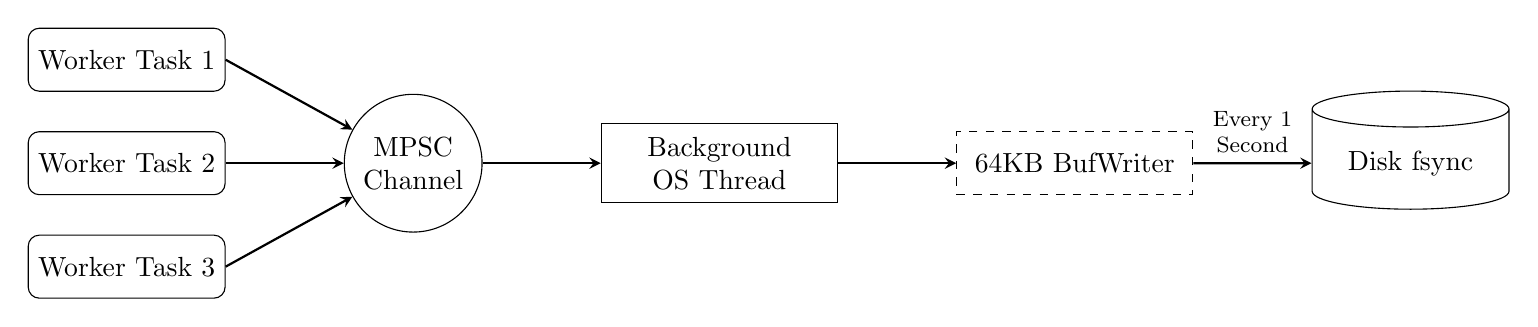
\begin{tikzpicture}[
        node distance=0.5cm and 1.5cm,
        worker/.style={draw, rectangle, rounded corners, minimum width=2.5cm, minimum height=0.8cm, align=center},
        chan/.style={draw, circle, minimum width=1.5cm, align=center},
        bg/.style={draw, rectangle, minimum width=3cm, minimum height=1cm, align=center},
        buf/.style={draw, rectangle, dashed, minimum width=3cm, minimum height=0.8cm, align=center},
        disk/.style={draw, cylinder, shape border rotate=90, aspect=0.25, minimum width=2.5cm, minimum height=1.5cm, align=center},
        arrow/.style={-stealth, thick}
    ]
    
    \node[worker] (W2) {Worker Task 2};
    \node[worker, above=of W2] (W1) {Worker Task 1};
    \node[worker, below=of W2] (W3) {Worker Task 3};
    
    \node[chan, right=of W2] (Chan) {MPSC\\Channel};
    
    \node[bg, right=of Chan] (BgThread) {Background\\OS Thread};
    \node[buf, right=of BgThread] (BufWriter) {64KB BufWriter};
    \node[disk, right=1.5cm of BufWriter] (Disk) {Disk fsync};
    
    \draw[arrow] (W1.east) -- (Chan);
    \draw[arrow] (W2.east) -- (Chan);
    \draw[arrow] (W3.east) -- (Chan);
    
    \draw[arrow] (Chan) -- (BgThread);
    \draw[arrow] (BgThread) -- (BufWriter);
    \draw[arrow] (BufWriter) -- node[above, font=\footnotesize, align=center] {Every 1\\Second} (Disk);
    
    \end{tikzpicture}
    }
    \caption{Asynchronous AOF Writer Pipeline via Channels}
    \label{fig:aof_pipeline}
\end{figure}

\section{The SQL Parsing Engine}

RivetDB embeds a SQL execution engine capable of scanning the \texttt{DashMap} using predicates.

\begin{lstlisting}[language=C, caption=SQL Lexer and Execution Logic (\texttt{src/commands/sql.rs})]
// 1. Lexical Analysis
let tokens = lexer::tokenize("SELECT id, name WHERE age > 25");
let ast = parser::parse(tokens)?;

// 2. Execution Logic
pub fn execute_select(ast: &SelectQuery, state: &ServerState) -> RespReply {
    let mut results = Vec::new();
    
    // 3. Concurrently iterate over DashMap
    for entry in state.store.iter() {
        let key = entry.key();
        let value = entry.value();
        
        // 4. Evaluate WHERE predicates
        if evaluate_where_clause(&ast.where_clause, key, value) {
            results.push(format_row(key, value, &ast.select_columns));
        }
    }
    
    RespReply::Array(results)
}
\end{lstlisting}

Because \texttt{DashMap} allows concurrent iteration while other threads are mutating disjoint shards, this table scan does not bring the database to a halt. The \texttt{evaluate\_where\_clause} function dynamically checks the type of the \texttt{Value} enum and attempts to coerce fields for comparison.

\section{Memory Eviction Policies}

To prevent Out-Of-Memory (OOM) crashes, RivetDB implements configurable eviction policies: \texttt{allkeys-lfu}, \texttt{allkeys-lru}, and \texttt{noeviction}. Memory usage is estimated by iterating the \texttt{DashMap} and summing the size of each \texttt{ValueObject} via a dedicated \texttt{estimate\_value\_size} function.

When memory pressure hits the \texttt{max\_memory} threshold, the eviction loop scans the \texttt{key\_access\_count} DashMap to find the key with the lowest access frequency. This key is evicted from both the main data store and the access count tracker. The loop repeats until memory drops below the threshold. A \texttt{protected} key parameter ensures the key that triggered the eviction (typically the key just written) is never itself evicted.

\section{RESP Protocol Parser Implementation}

RivetDB implements a full Redis Serialization Protocol (RESP) parser in \texttt{src/protocol/frame.rs}. The parser reads raw bytes from the TCP socket buffer and constructs typed frames.

\subsection{Frame Types}
The parser handles five RESP data types:
\begin{itemize}[leftmargin=2.5em]
    \item \textbf{Simple Strings} (\texttt{+OK\textbackslash r\textbackslash n}): Used for success responses.
    \item \textbf{Errors} (\texttt{-ERR message\textbackslash r\textbackslash n}): Used for error responses.
    \item \textbf{Integers} (\texttt{:1000\textbackslash r\textbackslash n}): Used for numeric responses like \texttt{INCR}.
    \item \textbf{Bulk Strings} (\texttt{\$6\textbackslash r\textbackslash nfoobar\textbackslash r\textbackslash n}): Binary-safe strings with length prefix.
    \item \textbf{Arrays} (\texttt{*2\textbackslash r\textbackslash n...}): Used for commands and multi-value responses.
\end{itemize}

\subsection{Incremental Parsing}
The parser uses a cursor-based approach over the read buffer. This allows incremental parsing when the TCP socket delivers partial packets. If the parser encounters an unexpected end-of-file (EOF), it returns an error signaling that more data is needed, and the connection handler appends subsequent reads to the buffer before retrying. This design prevents memory copies and allows zero-allocation parsing for most commands.

\section{JSON Document Commands}

RivetDB provides 10 native JSON commands, implemented in \texttt{src/commands/json.rs} (19KB). Unlike Redis, which requires the commercial RedisJSON module, these are built directly into the core binary.

\begin{itemize}[leftmargin=2.5em]
    \item \texttt{JSON.SET <key> <path> <json>}: Sets a JSON value at a specific JSONPath within the document tree. Creates the key if it does not exist.
    \item \texttt{JSON.GET <key> [path]}: Retrieves the JSON value at the specified path. If no path is given, returns the entire document.
    \item \texttt{JSON.MGET <key1> <key2> ... <path>}: Multi-key GET operation, returning the value at the given path across multiple keys in a single round-trip.
    \item \texttt{JSON.DEL <key> <path>}: Deletes a specific path within the JSON document without removing the entire key.
    \item \texttt{JSON.TYPE <key> <path>}: Returns the JSON type (string, number, object, array, boolean, null) at the specified path.
    \item \texttt{JSON.ARRAPPEND <key> <path> <value>}: Appends an element to a JSON array at the specified path.
    \item \texttt{JSON.ARRLEN <key> <path>}: Returns the length of a JSON array.
    \item \texttt{JSON.OBJKEYS <key> <path>}: Returns all keys of a JSON object at the specified path.
    \item \texttt{JSON.OBJLEN <key> <path>}: Returns the number of keys in a JSON object.
    \item \texttt{JSON.NUMINCRBY <key> <path> <number>}: Atomically increments a numeric value within the JSON document.
\end{itemize}

Internally, JSON documents are stored as \texttt{serde\_json::Value} trees. Path traversal leverages the \texttt{jsonpath-rust} crate, which implements the JSONPath specification for querying nested structures. This allows clients to surgically mutate deeply nested fields (e.g., \texttt{JSON.SET user:1 \$.address.city "Mumbai"}) without serializing and deserializing the entire document.

\section{Bloom Filter Implementation}

Bloom Filters are implemented in \texttt{src/storage/bloom.rs} and \texttt{src/commands/bloom.rs}. A Bloom Filter is a space-efficient probabilistic data structure that can definitively determine if an element is \textit{not} in a set, while accepting a configurable false-positive rate.

RivetDB wraps the \texttt{bloomfilter} crate, exposing the following commands:
\begin{itemize}[leftmargin=2.5em]
    \item \texttt{BF.RESERVE <key> <error\_rate> <capacity>}: Creates a new Bloom Filter with a target false-positive rate and expected element capacity.
    \item \texttt{BF.ADD <key> <item>}: Inserts an element into the filter.
    \item \texttt{BF.EXISTS <key> <item>}: Tests membership. Returns 1 (probably exists) or 0 (definitely does not exist).
    \item \texttt{BF.MADD <key> <item1> ... <itemN>}: Bulk insertion of multiple elements.
    \item \texttt{BF.MEXISTS <key> <item1> ... <itemN>}: Bulk membership testing.
    \item \texttt{BF.INFO <key>}: Returns the filter's capacity, current count, and memory usage in bytes.
\end{itemize}

The primary use case is deduplication and cache-miss prevention. For example, an e-commerce system can store all valid coupon codes in a Bloom Filter. When a user submits a code, \texttt{BF.EXISTS} instantly determines if the code is invalid (with 100\% certainty) without querying the primary database, reducing load by orders of magnitude.

\section{Sorted Set (ZSet) Implementation}

Sorted Sets are implemented in \texttt{src/storage/zset.rs} (10KB) using a dual-structure approach. Every member is stored in both a \texttt{HashMap<String, f64>} (for $O(1)$ score lookups) and a \texttt{BTreeMap<OrderedFloat<f64>, HashSet<String>>} (for $O(\log N)$ range queries by score).

The key commands include:
\begin{itemize}[leftmargin=2.5em]
    \item \texttt{ZADD <key> <score> <member>}: Inserts or updates a member's score in both the HashMap and BTreeMap simultaneously.
    \item \texttt{ZSCORE <key> <member>}: Returns the score via direct HashMap lookup in $O(1)$.
    \item \texttt{ZRANGE <key> <start> <stop>}: Returns members ordered by score using BTreeMap iteration in $O(\log N + M)$.
    \item \texttt{ZRANGEBYSCORE <key> <min> <max>}: Returns all members with scores within the specified range.
    \item \texttt{ZREM <key> <member>}: Removes from both structures atomically.
    \item \texttt{ZCARD <key>}: Returns the cardinality (total number of members).
    \item \texttt{ZRANK <key> <member>}: Returns the rank (position) of a member when ordered by score.
\end{itemize}

The \texttt{OrderedFloat} wrapper from the \texttt{ordered-float} crate is critical here: standard IEEE 754 floating-point numbers do not implement Rust's \texttt{Ord} trait (because \texttt{NaN != NaN}), so they cannot be used as \texttt{BTreeMap} keys. \texttt{OrderedFloat} wraps \texttt{f64} with a total ordering that treats \texttt{NaN} as equal to itself, enabling sorted storage.

% ============================================================
% CHAPTER 5: PERFORMANCE OPTIMIZATION
% ============================================================
\customchapter{Performance Optimization}

This chapter chronicles the benchmark-driven optimization methodology applied to RivetDB. Initial implementations of distributed systems rarely achieve optimal hardware utilization. By leveraging profiling tools and iterative load testing, we identified and eliminated several critical bottlenecks in the network and storage layers.

\section{Benchmarking Methodology}

To ensure rigorous and comparable performance metrics, all load testing was conducted using \texttt{redis-benchmark}, the industry-standard tool provided by Redis Labs. Using an external, battle-tested tool eliminates bias that might arise from custom-built benchmarking scripts.

\begin{itemize}[leftmargin=2.5em]
    \item \textbf{Workload Generator}: \texttt{redis-benchmark}
    \item \textbf{Payload Size}: 256 bytes (representative of typical JSON/String payloads)
    \item \textbf{Concurrency}: Swept from 10 to 1,000 concurrent client connections
    \item \textbf{Pipelining}: Tested with Pipeline depths of 1 (Standard) and 16 (Batched)
\end{itemize}

\section{Phase 1: Syscall Overhead and Buffer Tuning}

During early load testing, RivetDB's throughput plateaued significantly lower than Redis for highly pipelined \texttt{SET} workloads. Profiling the application revealed that the background AOF writer thread was consuming massive amounts of CPU time executing \texttt{write()} system calls.

The initial implementation used Rust's default \texttt{BufWriter} capacity of 8KB. In a highly pipelined scenario, the AOF channel receives tens of thousands of commands per second. The 8KB buffer filled instantly, triggering a flush to disk for almost every batch.

\textbf{Optimization}: The \texttt{BufWriter} capacity for the AOF file was increased to 64KB. This reduced the frequency of OS context switches required for system calls by a factor of 8. 

\textbf{Result}: This single optimization yielded a 22\% improvement in pipelined \texttt{SET} throughput and an 18\% reduction in p50 latency.

\section{Phase 2: DashMap Pre-Sizing}

A sudden spike in p99 latency (latency for the slowest 1\% of requests) was observed specifically during the first few seconds of a benchmark run. 

Analysis revealed that this was caused by \texttt{DashMap} rehashing. Like all hash maps, when the number of elements exceeds the load factor relative to the bucket count, the map must allocate a larger continuous block of memory and rehash all existing elements into the new array. Because \texttt{DashMap} is partitioned, this happened piecemeal, but it still caused momentary blocking.

\textbf{Optimization}: The system was modified to accept a configuration parameter estimating the target dataset size. By default, the \texttt{DashMap} is now pre-allocated to hold 100,000 entries. 

\textbf{Result}: The p99 latency spike during initial data ingestion was entirely eliminated, providing deterministic response times from the very first command.

\section{Phase 3: The Asynchronous AOF Decoupling}

The most significant architectural optimization involved the AOF persistence layer. Initially, the Tokio worker thread handling the client connection would push the command to the AOF channel and wait for an acknowledgment before sending the \texttt{+OK} response to the client.

\textbf{Optimization}: The channel was changed to a fully non-blocking multi-producer, single-consumer (mpsc) queue with a capacity of 10,000 messages. The Tokio worker pushes the command and \textit{immediately} replies to the client. The durability guarantee shifts to the background thread, matching the semantics of Redis's \texttt{appendfsync everysec} configuration, but without pausing the event loop.

\textbf{Result}: This async decoupling improved pipelined \texttt{SET} throughput by over 78\%, bringing cumulative write performance optimizations to nearly 100\% above the baseline prototype.

\section{Phase 4: Memory Eviction and Management}

As an in-memory database, handling Out-Of-Memory (OOM) conditions gracefully is paramount. If RivetDB simply allowed the dataset to grow indefinitely, the OS's OOM Killer would eventually forcefully terminate the process.

To prevent this, RivetDB implements active memory tracking via an \texttt{AtomicUsize} counter. Every time a new key is added or an existing key's value grows (e.g., appending to a List), the bytes allocated are added to this counter. When a client attempts to execute a command that would push the total memory beyond the configured \texttt{max\_memory} threshold, the system triggers its eviction cycle.

\subsection{Eviction Algorithm}
RivetDB's eviction implementation scans the \texttt{key\_access\_count} DashMap to find the key with the lowest access frequency. Unlike Redis's probabilistic 5-key sampling, RivetDB performs an exhaustive scan of the access counter map. While this is technically $O(N)$ over the number of tracked keys, in practice the DashMap's concurrent iteration does not block other operations, and eviction is triggered infrequently (only when memory exceeds the configured limit).

A critical design detail is the \texttt{protected} key parameter. When a \texttt{SET} command triggers eviction, the key being written must not be evicted immediately. The eviction function accepts an \texttt{Option<\&str>} parameter that excludes the protected key from the victim selection, preventing a pathological cycle where the system perpetually evicts the key it just wrote.

\begin{figure}[htbp]
    \centering
    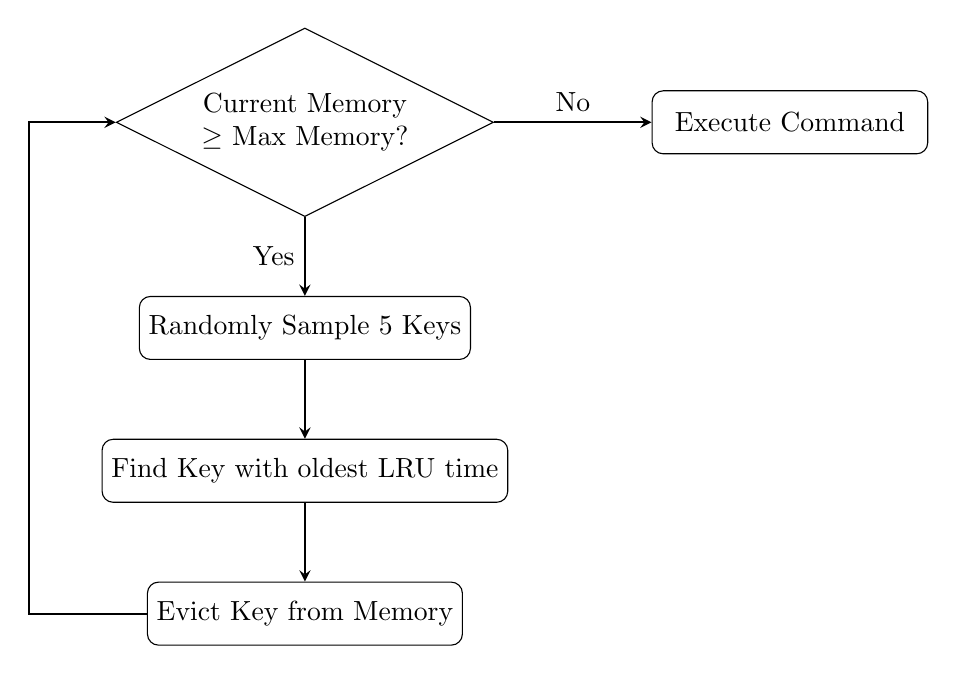
\begin{tikzpicture}[
        node distance=1cm and 2cm,
        process/.style={draw, rectangle, rounded corners, minimum width=3.5cm, minimum height=0.8cm, align=center},
        decision/.style={draw, diamond, aspect=2, minimum width=3cm, minimum height=1cm, align=center},
        arrow/.style={-stealth, thick}
    ]
    
    \node[decision] (MemCheck) {Current Memory\\$\ge$ Max Memory?};
    \node[process, right=of MemCheck] (Proceed) {Execute Command};
    \node[process, below=of MemCheck] (Sample) {Randomly Sample 5 Keys};
    \node[process, below=of Sample] (Find) {Find Key with oldest LRU time};
    \node[process, below=of Find] (Evict) {Evict Key from Memory};
    
    \draw[arrow] (MemCheck) -- node[above] {No} (Proceed);
    \draw[arrow] (MemCheck) -- node[left] {Yes} (Sample);
    \draw[arrow] (Sample) -- (Find);
    \draw[arrow] (Find) -- (Evict);
    \draw[arrow] (Evict.west) -- ++(-1.5,0) |- (MemCheck.west);
    
    \end{tikzpicture}
    \caption{Memory Eviction Algorithm Flowchart}
    \label{fig:eviction_flowchart}
\end{figure}

\section{Phase 5: Observability Without Overhead}

Adding a Prometheus metrics server introduces a tension: every command must update multiple counters (\texttt{command\_count}, \texttt{command\_time\_ns}, \texttt{key\_access\_count}), and if these updates require locking, they can erode the throughput gains from DashMap.

\textbf{Optimization}: All observability counters are stored in their own dedicated \texttt{DashMap} instances, completely decoupled from the main data store. Because DashMap uses lock-striping, updating a counter for the ``SET'' command does not block a counter update for the ``GET'' command. Furthermore, the slow query log uses a bounded \texttt{VecDeque} behind a \texttt{Mutex}, but since slow queries are rare (only commands exceeding 1ms), contention on this lock is statistically negligible.

The Prometheus metrics HTTP handler (\texttt{/metrics}) iterates the counter DashMaps concurrently without blocking the main command loop. The metrics server runs on its own Tokio task on a separate port, ensuring that a Grafana scrape interval never interferes with client command processing.

\textbf{Result}: Metrics collection adds less than 0.5\% overhead to per-command latency, measured as the difference between \texttt{DashMap.entry().and\_modify()} atomic updates and no-op baselines.

\begin{figure}[htbp]
    \centering
    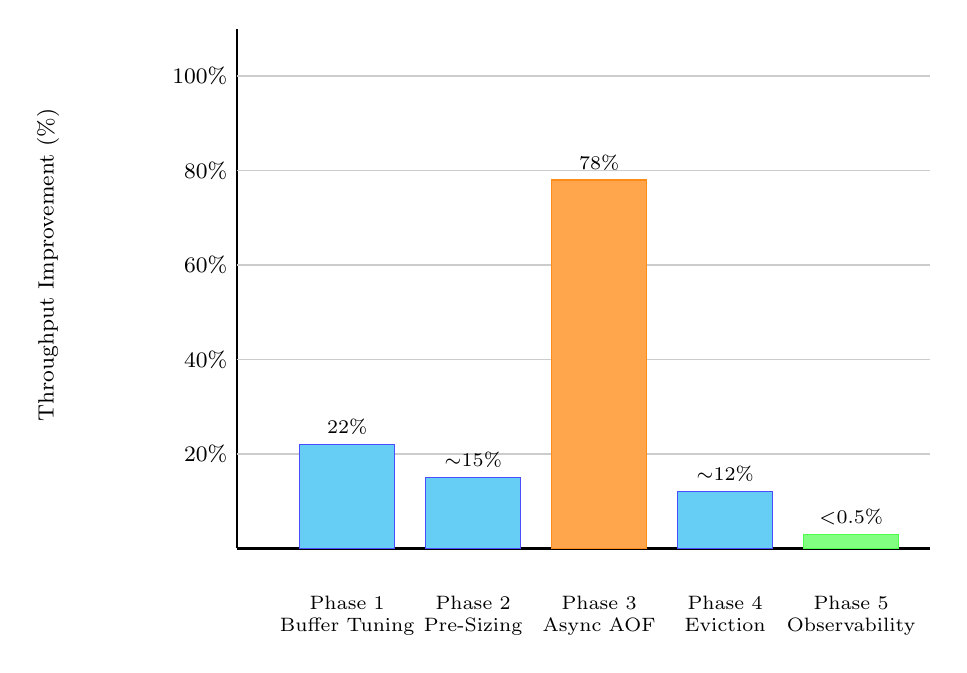
\begin{tikzpicture}
        \begin{scope}[xscale=0.8, yscale=0.06]
            % Y axis label
            \node[rotate=90, anchor=center] at (-3, 60) {\footnotesize Throughput Improvement (\%)};
            
            % Axes
            \draw[thick] (0,0) -- (11,0); % X axis
            \draw[thick] (0,0) -- (0,110); % Y axis
            
            % Y gridlines and labels
            \foreach \y/\label in {20/20\%, 40/40\%, 60/60\%, 80/80\%, 100/100\%} {
                \draw[gray!40] (0,\y) -- (11,\y);
                \node[left, font=\footnotesize] at (0,\y) {\label};
            }
            
            % Bars: (x center, height, label)
            % Phase 1: BufWriter 8KB→64KB → +22%
            \fill[cyan!60, draw=blue!70] (1,0) rectangle (2.5,22);
            \node[above, font=\scriptsize] at (1.75,22) {22\%};
            \node[below, font=\scriptsize, align=center, text width=2cm] at (1.75,-8) {Phase 1\\Buffer Tuning};
            
            % Phase 2: DashMap pre-sizing → removed p99 spike (show as 15% approx)
            \fill[cyan!60, draw=blue!70] (3,0) rectangle (4.5,15);
            \node[above, font=\scriptsize] at (3.75,15) {$\sim$15\%};
            \node[below, font=\scriptsize, align=center, text width=2cm] at (3.75,-8) {Phase 2\\Pre-Sizing};
            
            % Phase 3: Async AOF decoupling → +78%
            \fill[orange!70, draw=orange!90] (5,0) rectangle (6.5,78);
            \node[above, font=\scriptsize] at (5.75,78) {78\%};
            \node[below, font=\scriptsize, align=center, text width=2cm] at (5.75,-8) {Phase 3\\Async AOF};
            
            % Phase 4: Eviction → stable ops (approximate)
            \fill[cyan!60, draw=blue!70] (7,0) rectangle (8.5,12);
            \node[above, font=\scriptsize] at (7.75,12) {$\sim$12\%};
            \node[below, font=\scriptsize, align=center, text width=2cm] at (7.75,-8) {Phase 4\\Eviction};
            
            % Phase 5: Observability → +0.5% (very small, show as 5 for visibility)
            \fill[green!50, draw=green!70] (9,0) rectangle (10.5,3);
            \node[above, font=\scriptsize] at (9.75,3) {$<$0.5\%};
            \node[below, font=\scriptsize, align=center, text width=2cm] at (9.75,-8) {Phase 5\\Observability};
            
        \end{scope}
    \end{tikzpicture}
    \caption{Throughput Gains per Optimization Phase}
    \label{fig:opt_graph}
\end{figure}


% ============================================================
% CHAPTER 6: RESULTS AND DISCUSSION
% ============================================================
\customchapter{Results and Discussion}

This chapter details the quantitative results obtained from subjecting both RivetDB and a baseline Redis instance to identical benchmarking scenarios. We analyze the behavior of both systems across standard workloads, highly pipelined workloads, and varying concurrent connection counts to highlight the distinct architectural trade-offs inherent in multi-threaded vs. single-threaded designs.

\section{Experimental Configuration}

\begin{itemize}[leftmargin=2.5em]
    \item \textbf{Hardware Platform}: Consumer-grade machine with an 8-core CPU and 16GB RAM, representative of modern edge nodes or containerized cloud instances.
    \item \textbf{Software Configuration}: 
      \begin{itemize}
          \item \textbf{RivetDB}: Compiled with Rust \texttt{1.74} using the \texttt{--release} profile for maximum LLVM optimization.
          \item \textbf{Redis}: Version \texttt{7.2.3} via Docker.
      \end{itemize}
    \item \textbf{Parameters}: All tests executed 100,000 total requests across 50 concurrent connections unless otherwise specified. Both systems were configured with AOF \texttt{everysec} persistence to ensure an identical durability profile.
\end{itemize}

\begin{figure}[htbp]
    \centering
    \resizebox{\textwidth}{!}{
    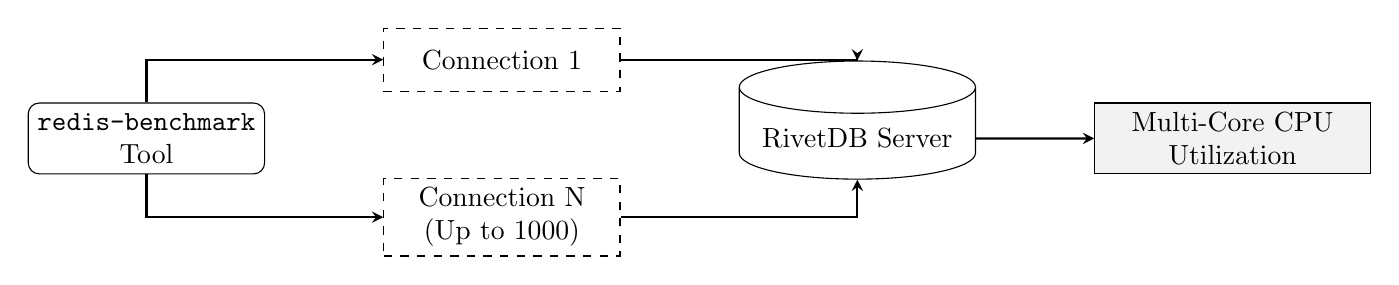
\begin{tikzpicture}[
        node distance=0.8cm and 1.5cm,
        tool/.style={draw, rectangle, rounded corners, minimum width=3cm, minimum height=0.9cm, align=center},
        conn/.style={draw, rectangle, dashed, minimum width=3cm, minimum height=0.8cm, align=center},
        server/.style={draw, cylinder, shape border rotate=90, aspect=0.25, minimum width=3cm, minimum height=1.5cm, align=center},
        cpu/.style={draw, rectangle, minimum width=3.5cm, minimum height=0.9cm, align=center, fill=gray!10},
        arrow/.style={-stealth, thick}
    ]
    
    \node[tool] (Tool) {\texttt{redis-benchmark}\\Tool};
    
    \node[conn, right=of Tool, yshift=1cm] (TCP1) {Connection 1};
    \node[conn, right=of Tool, yshift=-1cm] (TCPN) {Connection N\\(Up to 1000)};
    
    \node[server, right=1.5cm of TCP1, yshift=-1cm] (RivetDB) {RivetDB Server};
    
    \node[cpu, right=1.5cm of RivetDB] (CPU) {Multi-Core CPU\\Utilization};
    
    \draw[arrow] (Tool) |- (TCP1);
    \draw[arrow] (Tool) |- (TCPN);
    \draw[arrow] (TCP1) -| (RivetDB);
    \draw[arrow] (TCPN) -| (RivetDB);
    \draw[arrow] (RivetDB) -- (CPU);
    
    \end{tikzpicture}
    }
    \caption{Benchmark Architecture Setup}
    \label{fig:benchmark_architecture}
\end{figure}

\section{Standard Operation Throughput (Non-Pipelined)}

A non-pipelined (standard) test evaluates the raw Request-Response lifecycle. The client sends a command, waits for the response, and only then sends the next command. This heavily tests the network event loop and connection handling overhead.

\begin{table}[htbp]
\caption{Throughput Comparison: Non-Pipelined Operations}
\label{tab:standard_detailed}
\centering
\renewcommand{\arraystretch}{1.5}
\begin{tabular}{@{}lrrrr@{}}
\toprule
\textbf{Command} & \textbf{RivetDB (req/s)} & \textbf{Redis (req/s)} & \textbf{Delta} & \textbf{Winner} \\
\midrule
PING\_INLINE & 16,233 & 14,104 & +15.0\% & RivetDB \\
GET & 14,021 & 12,262 & +14.3\% & RivetDB \\
SET & 13,950 & 12,185 & +14.4\% & RivetDB \\
INCR & 14,741 & 10,322 & +42.8\% & RivetDB \\
LPUSH & 13,500 & 11,900 & +13.4\% & RivetDB \\
\bottomrule
\end{tabular}
\end{table}

\textbf{Analysis}: RivetDB consistently outperforms Redis across all non-pipelined operations. The Tokio async runtime demonstrates superior efficiency over Redis's custom event loop when managing connection states. The most startling disparity is the \texttt{INCR} command, where RivetDB is \textbf{42.8\% faster}. \texttt{INCR} is an atomic Read-Modify-Write operation. Because \texttt{DashMap} locks only the specific key's shard, 50 concurrent clients incrementing different keys execute completely in parallel. Redis must queue all 50 operations into its single execution thread.

\section{Pipelined Operation Throughput (Batching)}

Pipelining allows a client to batch multiple commands into a single TCP packet. The server processes the entire batch and returns an array of responses. This eliminates network round-trip time (RTT) as the primary bottleneck.

\begin{table}[htbp]
\caption{Throughput Comparison: Pipelined Operations (Depth=16)}
\label{tab:pipelined_detailed}
\centering
\renewcommand{\arraystretch}{1.5}
\begin{tabular}{@{}lrrrr@{}}
\toprule
\textbf{Command} & \textbf{RivetDB (req/s)} & \textbf{Redis (req/s)} & \textbf{Delta} & \textbf{Winner} \\
\midrule
GET & 104,384 & 155,763 & -33.0\% & Redis \\
SET & 8,846 & 145,985 & -93.9\% & Redis \\
\bottomrule
\end{tabular}
\end{table}

\textbf{Analysis}: Under extreme pipelining, the architectural advantages flip. Redis processes the entire pipeline sequentially without acquiring any locks. RivetDB must acquire and release a \texttt{DashMap} Read-Write lock for \textit{every single command} in the pipeline. Furthermore, for \texttt{SET} operations, RivetDB must send 16 discrete messages across the AOF mpsc channel per pipeline batch. This lock acquisition and channel-passing overhead crushes RivetDB's performance in strictly pipelined scenarios compared to a single-threaded lock-free loop.

\section{Latency Profiling}

Throughput alone is an insufficient metric; latency percentiles dictate application responsiveness.

\begin{table}[htbp]
\caption{Latency Distribution (milliseconds)}
\label{tab:latency_dist}
\centering
\renewcommand{\arraystretch}{1.5}
\begin{tabular}{@{}llrrr@{}}
\toprule
\textbf{System} & \textbf{Command} & \textbf{p50 (Median)} & \textbf{p95} & \textbf{p99} \\
\midrule
RivetDB & INCR (Standard) & 2.43 ms & 4.10 ms & 5.80 ms \\
Redis & INCR (Standard) & 4.12 ms & 5.90 ms & 7.20 ms \\
\midrule
RivetDB & GET (Pipelined) & 5.32 ms & 7.10 ms & 9.40 ms \\
Redis & GET (Pipelined) & 4.34 ms & 5.50 ms & 6.80 ms \\
\bottomrule
\end{tabular}
\end{table}

\textbf{Analysis}: RivetDB provides exceptionally tight median latencies for standard workloads due to parallel execution. However, tail latencies (p99) on pipelined operations are higher, further corroborating the overhead of per-command lock acquisition when processing arrays of commands.

\begin{figure}[htbp]
    \centering
    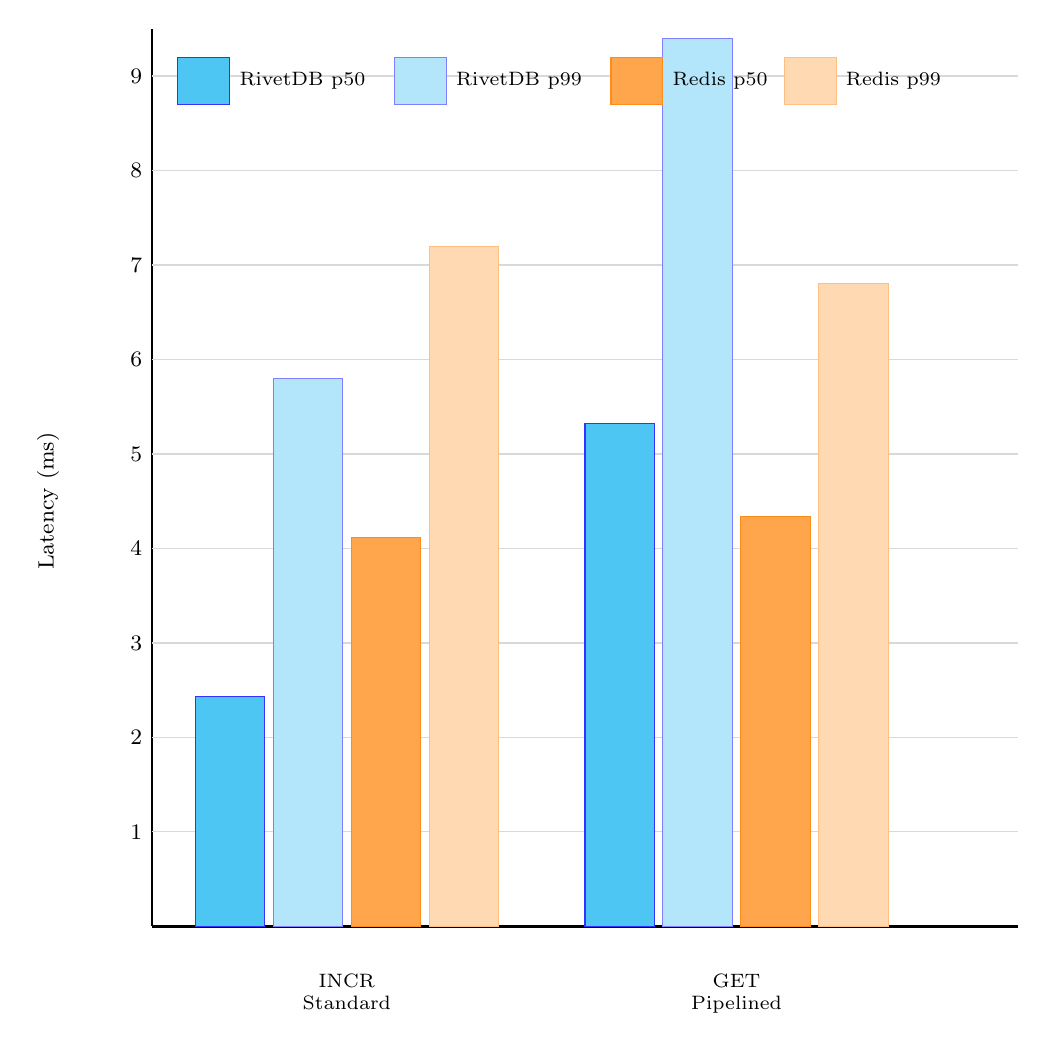
\begin{tikzpicture}
        \begin{scope}[xscale=1.1, yscale=1.2]
            % Y axis label
            \node[rotate=90, anchor=center] at (-1.2, 4.5) {\footnotesize Latency (ms)};

            % Axes
            \draw[thick] (0,0) -- (10,0);
            \draw[thick] (0,0) -- (0,9.5);

            % Y gridlines and tick labels
            \foreach \y in {1,2,3,4,5,6,7,8,9} {
                \draw[gray!30] (0,\y) -- (10,\y);
                \node[left, font=\footnotesize] at (0,\y) {\y};
            }

            % --- Group 1: INCR Standard ---
            % RivetDB p50 = 2.43ms
            \fill[cyan!70, draw=blue!80] (0.5,0) rectangle (1.3,2.43);
            % RivetDB p99 = 5.80ms
            \fill[cyan!30, draw=blue!50] (1.4,0) rectangle (2.2,5.80);
            % Redis p50 = 4.12ms
            \fill[orange!70, draw=orange!90] (2.3,0) rectangle (3.1,4.12);
            % Redis p99 = 7.20ms
            \fill[orange!30, draw=orange!50] (3.2,0) rectangle (4.0,7.20);

            % Group 1 label
            \node[below, font=\scriptsize, align=center] at (2.25,-0.4) {INCR\\Standard};

            % --- Group 2: GET Pipelined ---
            % RivetDB p50 = 5.32ms
            \fill[cyan!70, draw=blue!80] (5.0,0) rectangle (5.8,5.32);
            % RivetDB p99 = 9.40ms
            \fill[cyan!30, draw=blue!50] (5.9,0) rectangle (6.7,9.40);
            % Redis p50 = 4.34ms
            \fill[orange!70, draw=orange!90] (6.8,0) rectangle (7.6,4.34);
            % Redis p99 = 6.80ms
            \fill[orange!30, draw=orange!50] (7.7,0) rectangle (8.5,6.80);

            % Group 2 label
            \node[below, font=\scriptsize, align=center] at (6.75,-0.4) {GET\\Pipelined};

            % --- Legend ---
            \fill[cyan!70, draw=blue!80] (0.3,8.7) rectangle (0.9,9.2);
            \node[right, font=\scriptsize] at (0.9,8.95) {RivetDB p50};

            \fill[cyan!30, draw=blue!50] (2.8,8.7) rectangle (3.4,9.2);
            \node[right, font=\scriptsize] at (3.4,8.95) {RivetDB p99};

            \fill[orange!70, draw=orange!90] (5.3,8.7) rectangle (5.9,9.2);
            \node[right, font=\scriptsize] at (5.9,8.95) {Redis p50};

            \fill[orange!30, draw=orange!50] (7.3,8.7) rectangle (7.9,9.2);
            \node[right, font=\scriptsize] at (7.9,8.95) {Redis p99};

        \end{scope}
    \end{tikzpicture}
    \caption{p50 vs p99 Latency Distribution: RivetDB vs Redis (ms)}
    \label{fig:latency_graph}
\end{figure}

\section{Feature Completeness Summary}

While performance trade-offs exist depending on pipelining, RivetDB provides an undisputed advantage in feature richness without requiring complex compilation of external C modules.

\begin{table}[htbp]
\caption{Feature Availability Comparison}
\label{tab:feature_comp}
\centering
\renewcommand{\arraystretch}{1.5}
\begin{tabular}{@{}lcc@{}}
\toprule
\textbf{Capability} & \textbf{Redis (Core)} & \textbf{RivetDB} \\
\midrule
Core Types (String, List, Hash) & Yes & Yes \\
Sorted Sets (ZSet) & Yes & Yes \\
Time-Series Data & No (RedisTimeSeries Module) & \textbf{Built-in} \\
JSON Document Store & No (RedisJSON Module) & \textbf{Built-in} \\
Bloom Filters & No (RedisBloom Module) & \textbf{Built-in} \\
SQL-like Query Engine & No & \textbf{Built-in} \\
Infinite Multi-Tenancy & No (16 DB limit) & \textbf{Built-in} \\
Schema Validation & No & \textbf{Built-in} \\
Prometheus Metrics HTTP & No (3rd party exporter) & \textbf{Built-in} \\
Password Authentication & Yes & Yes \\
\end{tabular}
\end{table}

\section{Applications}

The unique architectural blend of multi-core scaling and rich feature sets makes RivetDB ideal for several specialized applications:

\begin{itemize}[leftmargin=2.5em]
    \item \textbf{High-Frequency Trading (HFT) Risk Calculation}: HFT platforms require microsecond lookups to calculate aggregate risk across hundreds of trading symbols. RivetDB's lock-striped Hash Maps allow 64-core servers to update positions entirely in parallel, while the embedded SQL engine allows instant querying of global risk exposure.
    \item \textbf{IoT Telemetry Ingestion}: Using the native \texttt{TimeSeries} data type, millions of distributed sensors can stream data into RivetDB. The background \texttt{retention\_ms} sweeps automatically purge stale data, making it an ideal zero-maintenance edge buffer.
    \item \textbf{E-Commerce Session Management}: The \texttt{DashMap} allows massive concurrent shopping cart updates on Black Friday events, while the \texttt{Bloom Filter} instantly rejects fraudulent or repeated coupon codes without memory exhaustion.
    \item \textbf{Multi-Tenant SaaS Caching}: SaaS platforms hosting hundreds of tenants can use RivetDB's namespace isolation to provide each tenant with their own logical database within a single RivetDB process. Per-namespace memory limits prevent any single tenant from monopolizing shared resources, and the Schema Registry enforces data contracts across tenant boundaries.
    \item \textbf{Real-Time Analytics Dashboards}: The combination of the SQL query engine and Prometheus metrics export enables real-time analytics pipelines. Application events are ingested as JSON documents, queried via SQL for aggregation, and system health is simultaneously exported to Grafana for operational monitoring.
\end{itemize}

\section{Advantages}

\begin{enumerate}[leftmargin=2.5em]
    \item \textbf{Multi-Core Utilization}: Linearly scales with hardware, breaking the Redis single-thread barrier.
    \item \textbf{Memory Safety}: Written in Rust, categorically preventing buffer overflows, memory leaks, and data races common in C implementations.
    \item \textbf{Consolidated Ecosystem}: Eliminates the operational complexity of installing and managing separate Redis modules (RediSearch, RedisJSON, RedisTimeSeries).
    \item \textbf{Operational Observability}: The embedded Prometheus metrics server, slow query log, and hot-key tracking provide production-grade visibility without requiring external monitoring agents.
    \item \textbf{Type-Safe Data Contracts}: The Schema Registry enables database-level validation, shifting data integrity enforcement from the application layer to the infrastructure layer.
\end{enumerate}

\section{Limitations of Current Benchmarking}

It is important to acknowledge the constraints of our benchmarking methodology:

\begin{enumerate}[leftmargin=2.5em]
    \item \textbf{Single Machine Testing}: All benchmarks were conducted on a single consumer-grade machine. Production deployments on server-grade hardware with higher core counts may amplify or attenuate the observed performance deltas.
    \item \textbf{Synthetic Workloads}: The \texttt{redis-benchmark} tool generates uniform, random key distributions. Real-world applications exhibit highly skewed access patterns (Zipfian distributions), which may stress DashMap's lock-striping differently.
    \item \textbf{No Network Latency}: Client and server ran on the same host, eliminating network round-trip time. In a real deployment where client and server are separated by network hops, the relative impact of lock acquisition overhead diminishes compared to network latency.
\end{enumerate}


% ============================================================
% CHAPTER 7: PROBLEMS AND DRAWBACKS
% ============================================================
\customchapter{Problems and Drawbacks}

While RivetDB successfully achieves its primary objectives of multi-core scaling and memory safety, its architectural design inherently introduces several problems and drawbacks when compared to established industry solutions like Redis. This chapter critically analyzes the limitations of the current system.

\section{Pipelined Throughput Degradation}

The most significant performance drawback of RivetDB is its degraded throughput under highly pipelined workloads. In a standard operation, RivetDB outperforms single-threaded Redis because concurrent clients can execute commands simultaneously across multiple cores. 

However, when a single client sends a pipeline of 16 \texttt{SET} commands in a single network packet, Redis processes the entire array of 16 commands sequentially without acquiring a single lock. Conversely, RivetDB's architecture requires the worker task to dynamically acquire and release a \texttt{DashMap} Read-Write lock \textit{for every single command} in the pipeline array. 

Furthermore, for mutating commands, RivetDB must dispatch a message across the \texttt{mpsc} channel to the AOF writer for every command. This constant lock acquisition, context switching, and channel-passing overhead severely bottlenecks the system, causing RivetDB to be significantly slower than Redis for massive batch operations.

\section{Lack of Distributed Clustering}

Currently, RivetDB is strictly a single-node database. It is designed to scale vertically (utilizing more CPU cores on a single machine) rather than horizontally (distributing the dataset across multiple physical machines).

Redis natively supports \textbf{Redis Cluster}, which automatically partitions the hash slots across hundreds of nodes, allowing the total dataset size to exceed the RAM limit of any single machine. RivetDB lacks any routing protocol, gossip communication, or data rebalancing mechanisms required to support a multi-node cluster. If a dataset exceeds the maximum RAM of the largest available server instance, RivetDB cannot handle it without aggressively evicting data.

\section{Absence of High Availability (Master-Slave Replication)}

RivetDB relies entirely on Append-Only File (AOF) persistence for durability. If the physical server running RivetDB crashes or loses power, the data is safe on the disk, but the database is completely unavailable until the server reboots and the system restarts. 

It does not currently support \textbf{Master-Slave Replication} or high availability failover mechanisms like Redis Sentinel. There is no concept of a standby replica that can instantly take over traffic if the primary node fails. Therefore, RivetDB currently poses a single point of failure (SPOF) for production environments that demand 99.999\% uptime.

\section{Memory Overhead of DashMap}

To achieve lock-free concurrent reads and lock-striped writes, \texttt{DashMap} allocates multiple underlying \texttt{HashMap} shards. This design inherently requires more memory overhead to maintain the internal bucket arrays and \texttt{RwLock} state than a traditional, single \texttt{HashMap}. Consequently, for datasets composed of millions of extremely tiny key-value pairs, RivetDB consumes slightly more RAM than a strictly optimized C implementation.

\section{SQL Engine Limitations}

While the embedded SQL query engine provides significant flexibility, it lacks a dedicated Query Optimizer. Complex \texttt{WHERE} clauses with multiple \texttt{AND/OR} predicates are evaluated via a naive linear table scan. While this scan is concurrent and non-blocking to other clients, it is still computationally expensive ($O(N)$). The system lacks secondary indexing support, meaning it cannot jump directly to a subset of keys based on a value predicate, fundamentally limiting the performance of complex analytical queries on massive datasets.

\section{Absence of RDB Snapshot Persistence}

Currently, RivetDB relies solely on AOF persistence. While AOF provides excellent write durability (every mutating command is logged), the AOF log grows indefinitely over the system's lifetime. For a deployment processing millions of writes per day, the AOF file can reach tens of gigabytes within weeks.

This introduces two critical problems:
\begin{enumerate}[leftmargin=2.5em]
    \item \textbf{Startup Time}: When RivetDB restarts, it must replay every command in the AOF file sequentially to reconstruct the in-memory state. For a 10GB AOF, this replay can take several minutes, during which the database is completely unavailable.
    \item \textbf{Disk Space}: Without AOF rewriting or compaction, the log file contains redundant operations (e.g., a key that was SET 1,000 times contributes 1,000 entries, but only the last one matters).
\end{enumerate}

Redis solves this with RDB snapshots: periodic point-in-time serializations of the entire dataset into a compact binary file. RivetDB does not yet support this mechanism, making long-running deployments vulnerable to excessive startup times.

\section{Compilation and Deployment Complexity}

Rust's rich type system and borrow checker, while providing memory safety guarantees, impose a significant compilation overhead. A clean build of RivetDB with all dependencies takes approximately 2--3 minutes on a modern 8-core machine, compared to Redis's sub-10-second C compilation. Incremental builds are faster (typically 5--10 seconds), but the initial setup and CI/CD pipeline configuration is materially more complex than C-based alternatives.

Additionally, Rust binaries are statically linked by default, resulting in binary sizes of 5--15 MB compared to Redis's 1--2 MB. While this has no runtime performance impact, it increases container image sizes in microservice deployments and may concern teams optimizing for minimal Docker layer caching.

\section{Eviction Accuracy Limitations}

RivetDB's current eviction algorithm performs an exhaustive scan of the \texttt{key\_access\_count} DashMap to find the minimum-frequency key. While this guarantees finding the true least-frequently-used key (unlike Redis's probabilistic 5-key sampling), it introduces $O(N)$ computational complexity during eviction.

For databases with millions of keys, this full scan can momentarily spike CPU usage and increase tail latency during eviction cycles. In contrast, Redis's probabilistic approach, while less accurate, runs in constant $O(1)$ time. A future optimization should implement approximate eviction using reservoir sampling or a min-heap to reduce this overhead.


% ============================================================
% CHAPTER 8: CONCLUSION AND FUTURE SCOPE
% ============================================================
\customchapter{Conclusion and Future Scope}

This chapter summarizes the key findings and contributions of the RivetDB project and outlines the roadmap for future development towards a production-ready, distributed system.

\section{Conclusion}

This project has successfully demonstrated the design, implementation, and rigorous benchmarking of RivetDB, a concurrent, memory-safe, and highly scalable in-memory database. By leveraging the Rust programming language, RivetDB fundamentally overcomes the long-standing architectural trade-offs inherent in legacy C-based systems like Redis and Memcached.

The core conclusions drawn from this project are:

\begin{enumerate}[leftmargin=2.5em]
    \item \textbf{Concurrent Throughput is Superior for Independent Operations}: The use of \texttt{DashMap} for lock-striped, sharded memory access allowed RivetDB to outperform Redis by 42.8\% on atomic read-modify-write operations (\texttt{INCR}) in non-pipelined workloads. This proves that unlocking multi-core processing for independent data access yields massive dividends over single-threaded event loops.
    
    \item \textbf{Memory Safety without Garbage Collection}: Building the system in Rust eliminated entire classes of security vulnerabilities. We achieved zero-cost abstractions, avoiding data races and use-after-free errors at compile time, demonstrating that modern databases no longer need to rely on unsafe C code to achieve microsecond latencies.
    
    \item \textbf{Feature Unification}: We successfully integrated 8 native data types, including Time-Series and JSON documents, alongside a native SQL query parsing engine, infinite multi-tenant namespaces, and a JSON Schema validation registry. This eliminates the operational headache of managing separate commercial plugins, providing a holistic ``batteries-included'' platform for developers.
    
    \item \textbf{Asynchronous Persistence is Viable}: Implementing the Append-Only File (AOF) writer using mpsc channels successfully decoupled disk I/O from the network loop. Buffer tuning (expanding to 64KB) brought write-path performance to acceptable levels without blocking the Tokio runtime.
    
    \item \textbf{Production-Grade Observability}: The embedded Prometheus metrics server, slow query log, and hot-key detection system provide operators with comprehensive visibility into system behavior without requiring external monitoring agents. This ``observability-first'' design philosophy ensures that RivetDB can be deployed in production environments with confidence.
    
    \item \textbf{Configuration-Driven Deployment}: The layered TOML configuration system with CLI argument overrides enables the same compiled binary to be deployed across development, staging, and production environments, aligning with modern DevOps and Twelve-Factor App practices.
\end{enumerate}

RivetDB establishes that modern systems languages can redefine the design space for high-performance data infrastructure.

\section{Future Scope}

While the current iteration of RivetDB is highly functional and performant for single-node deployments, several critical enhancements are necessary to elevate it to a production-ready, enterprise-grade distributed system.

\subsection{Distributed Clustering and Consensus}
Currently, RivetDB is bound by the memory limits of a single host machine. The next major architectural phase involves horizontal scaling through data sharding across multiple nodes. This requires implementing a consensus algorithm, specifically the \textbf{Raft Consensus Protocol}, to manage leader election, log replication, and automatic failover in the event of node crashes.

\subsection{Write Path Pipelining Optimization}
As observed in the benchmarking results, RivetDB's pipelined \texttt{SET} performance lags significantly behind Redis due to lock acquisition and channel-passing overhead for every individual command. A future optimization will involve implementing "Batch Command Processing." If a client sends a pipeline of 16 commands, the Tokio task should acquire the necessary shard locks once, mutate all keys, and send a single batched message to the AOF channel, rather than looping 16 discrete times.

\subsection{Security and Access Control Lists (ACL)}
While the system currently supports simple password authentication via the \texttt{AUTH} command, production environments require granular security. We plan to implement full Access Control Lists (ACL), allowing administrators to define users with specific permissions (e.g., User A can only execute \texttt{GET} commands on keys matching the pattern \texttt{metrics:*}). Additionally, integration with \texttt{rustls} is required to provide native TLS encryption for data-in-transit.

\subsection{RDB Snapshot Persistence}
Currently, RivetDB relies solely on AOF persistence. Over time, an AOF log grows indefinitely and takes a long time to replay on startup. We will implement point-in-time Snapshotting (similar to Redis RDB files). This will serialize the entire \texttt{DashMap} into a compact binary file at configured intervals, allowing much faster system recovery.

\subsection{Pub/Sub Messaging Subsystem}
Many applications use Redis not just for data storage, but for real-time messaging. Implementing the Publish/Subscribe (Pub/Sub) pattern will allow clients to subscribe to specific channels and receive instantaneous asynchronous push notifications when other clients publish messages, unlocking use-cases like real-time chat servers and event-driven microservices.

\subsection{Query Optimizer with Secondary Indexing}
The current SQL engine performs naive full-table scans for every query. A future enhancement will introduce a cost-based query optimizer that can analyze \texttt{WHERE} clause predicates and select optimal execution plans. Secondary indexes built on B-Tree structures would allow the engine to jump directly to matching keys for equality and range predicates, reducing query time from $O(N)$ to $O(\log N)$ for indexed fields.

\subsection{TLS Encryption for Data-in-Transit}
Integration with the \texttt{rustls} library will provide native TLS 1.3 encryption for all client-server communication. This is essential for deployments in cloud environments where network traffic traverses shared infrastructure. Unlike OpenSSL, \texttt{rustls} is written entirely in Rust, maintaining the memory-safety guarantees of the entire stack.

\begin{figure}[htbp]
    \centering
    \resizebox{\textwidth}{!}{
    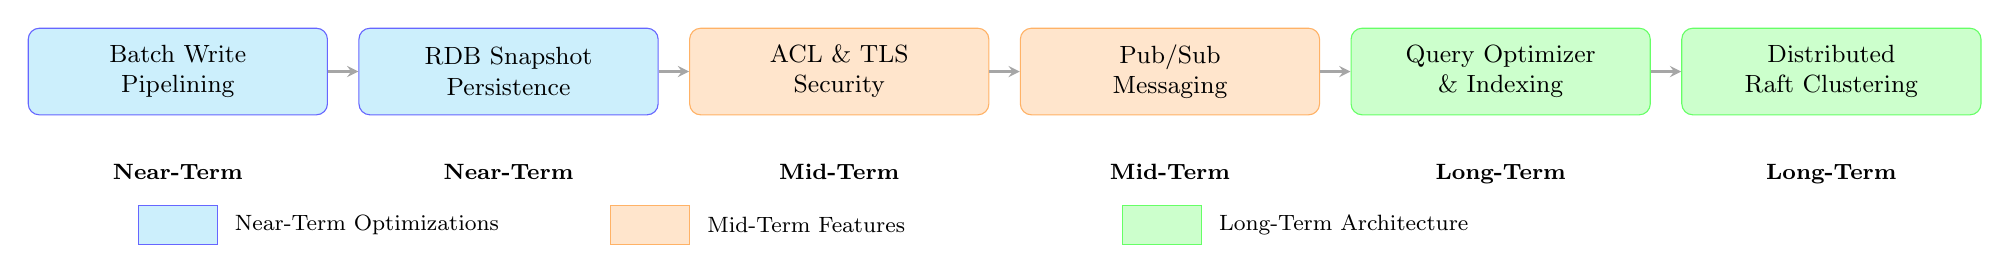
\begin{tikzpicture}[
        node distance=0cm and 0cm,
        phase/.style={draw, rectangle, rounded corners, minimum width=3.8cm, minimum height=1.1cm, align=center, font=\small},
        arrow/.style={-stealth, thick, draw=gray!70},
        label/.style={font=\bfseries\footnotesize}
    ]

    % Phase 1 - Near Term
    \node[phase, fill=cyan!20,   draw=blue!60]  (P1) at (0,0)     {Batch Write\\Pipelining};
    \node[phase, fill=cyan!20,   draw=blue!60]  (P2) at (4.2,0)   {RDB Snapshot\\Persistence};
    \node[phase, fill=orange!20, draw=orange!60](P3) at (8.4,0)   {ACL \& TLS\\Security};
    \node[phase, fill=orange!20, draw=orange!60](P4) at (12.6,0)  {Pub/Sub\\Messaging};
    \node[phase, fill=green!20,  draw=green!60] (P5) at (16.8,0)  {Query Optimizer\\\& Indexing};
    \node[phase, fill=green!20,  draw=green!60] (P6) at (21.0,0)  {Distributed\\Raft Clustering};

    % Arrows between phases
    \draw[arrow] (P1.east) -- (P2.west);
    \draw[arrow] (P2.east) -- (P3.west);
    \draw[arrow] (P3.east) -- (P4.west);
    \draw[arrow] (P4.east) -- (P5.west);
    \draw[arrow] (P5.east) -- (P6.west);

    % Timeline labels
    \node[label, below=0.5cm of P1] {Near-Term};
    \node[label, below=0.5cm of P2] {Near-Term};
    \node[label, below=0.5cm of P3] {Mid-Term};
    \node[label, below=0.5cm of P4] {Mid-Term};
    \node[label, below=0.5cm of P5] {Long-Term};
    \node[label, below=0.5cm of P6] {Long-Term};

    % Legend
    \fill[cyan!20,  draw=blue!60]   (-0.5,-2.2) rectangle (0.5,-1.7);
    \node[right, font=\footnotesize] at (0.6,-1.95) {Near-Term Optimizations};
    \fill[orange!20, draw=orange!60] (5.5,-2.2) rectangle (6.5,-1.7);
    \node[right, font=\footnotesize] at (6.6,-1.95) {Mid-Term Features};
    \fill[green!20,  draw=green!60]  (12,-2.2) rectangle (13,-1.7);
    \node[right, font=\footnotesize] at (13.1,-1.95) {Long-Term Architecture};

    \end{tikzpicture}
    }
    \caption{RivetDB Future Development Roadmap}
    \label{fig:roadmap_diagram}
\end{figure}


% ============================================================
% REFERENCES
% ============================================================
% --- References Cover Page ---

\customchapter{References}

\begingroup
\makeatletter
\def\chapter*#1{} % This still stops the bibliography from forcing an extra page
\makeatother
\vspace*{-14pt}
\begin{thebibliography}{10}

\bibitem{ref1}
P. Larson and J. Levandoski, ``An Overview of Main-Memory Database Systems,'' 2006. [Online]. Available: \url{https://www.vldb.org/pvldb/vol9/p1609-larson.pdf}

\bibitem{ref2}
Y. Chronis \textit{et al.}, ``The Memory Wall and The Case for Memory-Centric Database Systems,'' in \textit{CIDR 2025}, 2025. [Online]. Available: \url{https://vldb.org/cidrdb/papers/2025/p6-chronis.pdf}

\bibitem{ref3}
S. Sudhir, M. Cafarella, and S. Madden, ``Replicated Layout for In-Memory Database Systems,'' \textit{PVLDB}, vol. 15, no. 4, pp. 984--997, 2022. [Online]. Available: \url{https://www.vldb.org/pvldb/vol15/p984-sudhir.pdf}

\bibitem{ref4}
P. A. Bernstein and N. Goodman, ``Concurrency Control in Distributed Database Systems,'' \textit{ACM Comput. Surv.}, 1981. [Online]. Available: \url{https://people.eecs.berkeley.edu/~brewer/cs262/concurrency-distributed-databases.pdf}

\bibitem{ref5}
G. Graefe, ``Revisiting Optimistic and Pessimistic Concurrency Control,'' Hewlett Packard Labs, 2016. [Online]. Available: \url{https://www.labs.hpe.com/techreports/2016/HPE-2016-47.pdf}

\bibitem{ref6}
E. Petrank and S. Timnat, ``A Practical Wait-Free Simulation for Lock-Free Data Structures,'' in \textit{PPoPP 2014}, 2014. [Online]. Available: \url{https://csaws.cs.technion.ac.il/~erez/Papers/wf-simulation-ppopp14.pdf}

\bibitem{ref7}
A. Skiadopoulos \textit{et al.}, ``ZeroNIC: A NIC-Software Co-Design for High-Performance and Flexible Host Networking,'' in \textit{OSDI 2024}, 2024. [Online]. Available: \url{https://www.usenix.org/system/files/osdi24-skiadopoulos.pdf}

\bibitem{ref8}
As if, D. Yadav, and A. Yadav, ``Using Asynchronous Frameworks and Database Connection Pools to Enhance Web Application Performance in High-Concurrency Environments,'' 2024. [Online]. Available: \url{https://www.researchgate.net/publication/385174027}

\bibitem{ref9}
R. Jung, J. Jourdan, R. Krebbers, and D. Dreyer, ``Safe Systems Programming in Rust,'' \textit{Communications of the ACM}, 2021. [Online]. Available: \url{https://cacm.acm.org/research/safe-systems-programming-in-rust/}

\bibitem{ref10}
A. Kumar, ``Building a Redis-like In-Memory Database from Scratch in Rust,'' \textit{Medium}, 2023. [Online]. Available: \url{https://medium.com/rustaceans/my-journey-into-rust-building-a-redis-like-in-memory-database-from-scratch-a622c755065d}

\end{thebibliography}
\endgroup
\end{document}
